\chapter{Attosecond Transient-absorption Spectroscopy}
\label{chap:ATS}

\section{Introduction}
\label{sec:intro_ats}


\section{Autoionization resonances}
\label{sec:fano_ar}

One of the most extensively studied phenomenons using ATS has been autoionization of noble gas atoms in the time-domain \cite{wangAttosecondTimeResolvedAutoionization2010, ottAttosecondMultidimensionalInterferometry2012, stoossRealTimeReconstructionStrongFieldDriven2018, kaldunExtractingPhaseAmplitude2014, kaldunObservingUltrafastBuildup2016}.  Autoionization was first observed in 1935 by Beutler \cite{beutlerUeberAbsorptionsserienArgon1935} by studying photoabsorption of noble gas atoms, and it manifested itself as sharp, asymmetric peaks in the absorption spectrum.  These features were theoretically described by Fano in a seminal paper in 1961 \cite{fanoSulloSpettroDi1935, fanoEffectsConfigurationInteraction1961} as the result of interference between two pathways: direct ionization to the continuum and autoionization from a discrete state that is embedded in and coupled to the continuum. The theoretical framework that he developed can be treated as a more general formalism that describes interference between discrete and continuous pathways.\footnote{A very similar theory was independently developed by Feshbach in the context of nuclear physics, and these two theories have been unified by further theoretical work \cite{feshbachUnifiedTheoryNuclear1958, feshbachUnifiedTheoryNuclear1962, bhatiaLineshapeParameters1P1984}
	.} For this very reason, "Fano" resonances can be observed in a plethora of atomic, molecular, and condensed matter systems \cite{miroshnichenkoFanoResonancesNanoscale2010}.

\subsection{Autoionization in the frequency domain: Fano's original work}
\label{sec:og_fano}

As noted above, Fano's theoretical explanation of the photoabsorption spectrum observed by Beutler in noble gas atoms is based on interference between two pathways.  The relevant level diagram to describe this scenario is shown in figure \ref{fig:fano_level_diagram}, and specifically we will be considering the autoionization resonances in Ar because they will be used in the ATS experiments described in this chapter and in the following chapter.  In this case, there is a bound state $\ket{\psi_b}$ (one of the $3s3p^6np$ states in Ar) that is embedded within a set of continuum states $\ket{\psi_\varepsilon}$.  This entails that the energy of the bound state $E_b$ is degenerate with the energetic spectrum of continuum states. The coupling between the bound state $\ket{\psi_b}$ and the continuum $\ket{\psi_\varepsilon}$ through the configuration interaction leads to decay of the electron from the bound state to the continuum.  The following derivation of the photoabsorption cross section and phase follows closely from Fano's original paper and sources that have reproduced his original derivation \cite{fanoEffectsConfigurationInteraction1961, changFundamentalsAttosecondOptics2011, ottAttosecondMultidimensionalInterferometry2012}.

\begin{figure}
	\centering
	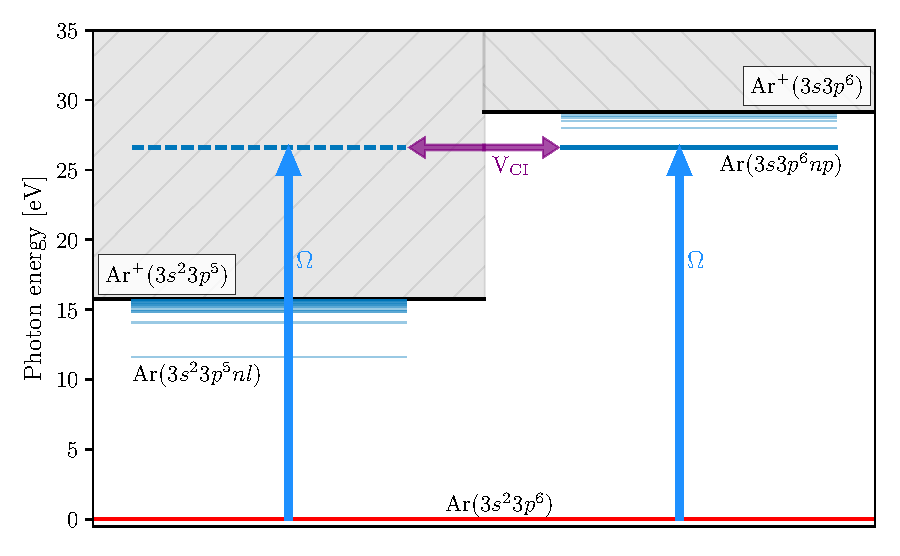
\includegraphics[width=0.8\textwidth]{figures/ATS/fano_level_diagram.pdf}
	\caption[Level diagram of Fano resonances in Argon]{Level diagram of argon showing the effect of autoionization states on XUV photoabsorption. There are two possible pathways for ionization with a photon of energy $\Omega$: (1) direct ionization to a continuum state (left side of figure) and (2) excitation to a bound state in the continuum (right side of figure).  In case (2), there is coupling between the bound state and the continuum through the configuration interaction.  This allows for the bound state to decay to the same continuum state as in case (1).  These effect leads to interference between these two pathways.}
	\label{fig:fano_level_diagram}
\end{figure}

The Hamiltonian describing this system can  be written as
\begin{equation}
\label{eqn:hamiltonian}
	\hat{H} = \hat{H_0} + \hat{V},
\end{equation}
where $\hat{H_0}$ is the zeroth order Hamiltonian and $\hat{V}$ is the correlation potential that describes the coupling between the discrete state $\ket{\psi_b}$ and the continuum state $\ket{\psi_\varepsilon}$.  The solutions to the zeroth order Hamiltonian are the continuum and bound states, such that 
\begin{align}
\label{eqn:configurations_hamiltonian}
	\hat{H_0}\ket{\psi_b} &= E_b\ket{\psi_b}\\
	\hat{H_0}\ket{\psi_\varepsilon} &= \varepsilon\ket{\psi_\varepsilon}
\end{align}
where the states $\ket{\psi_b}$ and $\ket{\psi_\varepsilon}$ are orthonormal.  These two solutions to the zeroth order Hamiltonian are referred to as configurations, and the interaction between them is given by $\hat{V}$. The coupling strength between these two configurations is given by the off-diagonal matrix element $V_\varepsilon$, such that
\begin{equation}
\label{eqn:coupling_matrix_element}
	\braket{\psi_\varepsilon|\hat{H}|\psi_b} = \braket{\psi_\varepsilon|\hat{H_0}+\hat{V}|\psi_b} = \braket{\psi_\varepsilon|\hat{V}|\psi_b} = V_\varepsilon.
\end{equation}  
This configuration interaction matrix element $V_\varepsilon$ depends upon the energy $\varepsilon$ and is generally a smooth function of the continuous energy $\varepsilon$.  Furthermore, the configuration interaction only couples different configurations and not within the same configuration.  The means that the diagonal matrix elements of $\hat{V}$ are zero,
\begin{align}
\label{eqn:config_int_diagonal}
	\braket{\psi_\varepsilon|\hat{V}|\psi_\varepsilon} &=0\\
	\braket{\psi_b|\hat{V}|\psi_b} &=0.
\end{align}
Therefore, the diagonal matrix elements of the full Hamiltonian in equation \ref{eqn:hamiltonian} are given by
\begin{align}
	\braket{\psi_\varepsilon|\hat{H}|\psi_\varepsilon} &= \varepsilon\delta(\varepsilon-\varepsilon')\\
	\braket{\psi_b|\hat{H}|\psi_b} &= E_b. 
\end{align}

Armed with these states as a basis, we can now expand an eigenstate of the full Hamiltonian $\hat{H}$.  This entails that the eigenstate $\ket{\Psi_E}$ of energy $E$, which is found by solving the equation
\begin{equation}
	\hat{H}\ket{\Psi_E}=E\ket{\Psi_E},
\end{equation}
can be expanded in this complete basis, such that
\begin{equation}
\label{eqn:eigenstate_expansion}
	\ket{\Psi_E} = a(E)\ket{\psi_b} + \int\diff\varepsilon'b(\varepsilon',E)\ket{\psi_{\varepsilon'}}.
\end{equation}
The physical interpretation of this expansion is that an electron at energy $E$ can originate from either the discrete state $\ket{\psi_b}$ or from the continuous state $\ket{\psi_\varepsilon}$.  The contribution from $\ket{\psi_\varepsilon}$ is direct ionization, and the contribution from $\ket{\psi_b}$ is autoionization (i.e. decay from the bound state $\ket{\psi_b}$ to the continuum).  The relative contributions of these two channels is given by the expansion coefficients $a(E)$ and $b(\varepsilon,E)$.

These expansion coefficients can be solved for and it involves algebra that is described in full detail in Fano's paper \cite{fanoEffectsConfigurationInteraction1961}.  The first step is to evaluate the relationship
\begin{equation}
	\braket{\Psi_E|\hat{H}|\Psi_E} = E
\end{equation}
using the expansion in eqn. \ref{eqn:eigenstate_expansion}.  This results in a system of two equations with the unknown coefficients $a(E)$ and $b(\varepsilon,E)$.  This system can be solved for analytical expressions of the expansion coefficients, and they are given by
\begin{align}
\label{eqn:expansion_coeff_a}
	a(E) &= \frac{\sin\Delta(E)}{\pi V_E}\\
\label{eqn:expansion_coeff_b}
	b(\varepsilon',E) &= \frac{V_{\varepsilon'}}{E-\varepsilon'}a(E)-\delta(\varepsilon'-E)\cos\Delta(E)
\end{align}
where
\begin{align}
\label{eqn:expansion_coeff_delta}
	\Delta(E) &= -\arctan\bigg(\frac{\pi\lvert V_E \rvert^2}{E-E_b-F(E)}\bigg)\\
\label{eqn:expansion_coeff_delta_F}
	F(E) &= \mathrm{PV}\int\diff\varepsilon'\frac{\lvert V_{\varepsilon'}\rvert^2}{E-\varepsilon'} 
\end{align}
and $\mathrm{PV}$ is the Cauchy principal value. The term  $F(E)$ is an energy-dependent shift of the bound state that depends upon the strength of the configuration interaction $\abs{V_{\varepsilon'}}^2$.  This shift can be either positive or negative, depending upon the sign of $\partial_{\varepsilon'}\abs{V_{\varepsilon'}}^2$ at $\varepsilon'=E$, where $\partial_{\varepsilon'}$ is the partial derivative with respect to $\varepsilon'$.  Thus, any change in  $V_{\varepsilon'}$ by an external field will lead to a shift in the resonance position.

Substituting the coefficients in equations \ref{eqn:expansion_coeff_a} and \ref{eqn:expansion_coeff_b} into equation \ref{eqn:eigenstate_expansion} yields
\begin{equation}
	\ket{\Psi_E}=\frac{\sin\Delta(E)}{\pi V_E}\ket{\psi_b}+\frac{\sin\Delta(E)}{\pi V_E}\bigg(\mathrm{PV}\int\diff\varepsilon'\frac{V_{\varepsilon'}}{E-\varepsilon'}\bigg)\ket{\psi_\varepsilon'}-\cos\Delta(E)\ket{\psi_E}.
\end{equation}
This can be further simplified by  introducing a modified discrete state given by
\begin{equation}
	\ket{\Phi} = \ket{\psi_b}+\mathrm{PV}\int\diff \varepsilon'\frac{V_\varepsilon'}{E-\varepsilon'}\ket{\psi_{\varepsilon'}},
\end{equation}
which allows us to express the eigenstate $\ket{\Psi_E}$ as
\begin{equation}
\label{eqn:eigen_with_a_b}
	\ket{\Psi_E}=\frac{\sin\Delta(E)}{\pi V_{E}}\ket{\Phi} - \cos\Delta(E)\ket{\psi_E}.
\end{equation}
Finally, the argument of equation \ref{eqn:expansion_coeff_delta_F} can be written in terms of an important parameter, the reduced energy given by
\begin{equation}
\label{eqn:normalized_eng}
	\epsilon = \frac{E-(E_b+F(E))}{\Gamma(E)/2} = \frac{E-E_\Phi}{\Gamma/2}
\end{equation}
where
\begin{equation}
	\Gamma(E) = 2\pi\abs{V_E}^2\approx\Gamma(E_b)=\Gamma.
\end{equation}
The interpretation of the modified bound state $\ket{\Phi}$ is that the configuration interaction is mixing the original discrete state $\ket{\psi_b}$ and the continuum states $\ket{\psi_\varepsilon'}$. So, for an energetic window near $E=E_\Phi$, one can consider the resonance energy to be $E_b$ and the resonance linewidth to be $\Gamma$.  Since $\Gamma=2\pi\abs{V_E}^2$, the resonance linewidth and the natural lifetime $h/\Gamma$ are directly related to the strength of the coupling between bound states and continuum states though the configuration interaction. Therefore, stronger (weaker) coupling would lead to faster (slower) decay from bound to continuum states, respectively.  From this, it can be seen that an external field that  is able to modify the strength of the configuration interaction, then that will lead to a change in the linewidth and position of the resonance.

Now that the eigenstates of the Hamiltonian $\hat{H}$ have been expanded, we will turn our attention to the photoabsorption spectrum.  In the original experiments done by Beutler, a sharp, asymmetric absorption profile was seen in the photoabsorption spectrum of noble gas atoms in the XUV \cite{beutlerUeberAbsorptionsserienArgon1935}.  From the expanded eigenstate given in equation \ref{eqn:eigen_with_a_b}, we can begin see how this asymmetric absorption profile might arise.  The coefficients in the expansion are proportional to sine and cosine functions of the reduced energy $\epsilon$, and, since they are odd and even functions of $\epsilon$, this will lead to constructive and destructive interference on either side of the resonance.  It is precisely this effect that will give rise to the asymmetric absorption lineshape.

To derive the photoabsorption spectrum, we will consider a transition from the ground state of the atom $\ket{g}$ by a XUV photon of energy $\Omega$.  This can be described through the use of the dipole transition operator
\begin{equation}
\label{eqn:dipole}
	\hat{D}=-e\mathbf{\hat{r}}\cdot\mathbf{E}_{XUV}(t)
\end{equation}
where $\mathbf{E}_{XUV}(t)$ is the electric field of the XUV.  Using this operator, the transition probability is given by the matrix element
\begin{equation}
\label{eqn:transition_me}
	\begin{aligned}
		\braket{\Psi_E|\hat{D}|g} &= \frac{1}{\pi V^*_{E}}\sin\Delta(E)\braket{\Phi|\hat{D}|g}-\cos\Delta(E)\braket{\psi_E|\hat{D}|g}\\
		&= \cos\Delta(E)\braket{\psi_E|\hat{D}|g}\Bigg[\tan\Delta(E)\frac{1}{\pi V^*_E}\frac{\braket{\Phi|\hat{D}|g}}{\braket{\psi_E|\hat{D}|g}} -1\Bigg].
	\end{aligned} 
\end{equation}
At this point, we can now introduce the well-known and important $q$ parameter, given by
\begin{equation}
\label{eqn:q-parameter}
	q(E) = \frac{1}{\pi V^*_E}\frac{\braket{\Phi|\hat{D}|g}}{\braket{\psi_E|\hat{D}|g}}\approx q(E_b)=q.
\end{equation}
The $q$ parameter describes the asymmetry of the resonance, and it is related to the ratio of transitions to the modified bound state $\ket{\Phi}$ and the continuum states $\ket{\psi_E}$.  Combining equations \ref{eqn:transition_me}, \ref{eqn:q-parameter}, and \ref{eqn:expansion_coeff_delta}, we arrive at
\begin{align}
	\braket{\Psi_E|\hat{D}|g} &=-\cos\Delta(E)\braket{\psi_E|\hat{D}|g}\Bigg[\frac{\pi\abs{V_E}^2}{E-(E_b+F(E))}q+1\Bigg]\\
	&=-\cos\Delta(E)\braket{\psi_E|\hat{D}|g}\Bigg[\frac{\Gamma/2}{E-(E_b+F(E))}q+1\Bigg],
\end{align}
and this can be further simplified using the reduced energy $\epsilon$, which yields
\begin{align}
	\braket{\Psi_E|\hat{D}|g} &= -\braket{\psi_E|\hat{D}|g}\cos\Delta(E)\bigg(\frac{q}{\epsilon}+1\bigg)\\
\label{eqn:fano_matirx_elements}
	\braket{\Psi_E|\hat{D}|g} &= \braket{\psi_E|\hat{D}|g}\frac{q+\epsilon}{\epsilon+i}.
\end{align}
Finally, using this relationship the ratio of transition probabilities can be calculated and leads to the well known Fano lineshape,
\begin{equation}
\label{eqn:transition_prob_ratio}
	\frac{\abs{\braket{\Psi_E|\hat{D}|g}}^2}{\abs{\braket{\psi_E|\hat{D}|g}}^2}=\frac{(q+\epsilon)^2}{\epsilon^2 + 1}.
\end{equation}
This ratio is proportional to the photoabsorption cross section, and is plotted for various $q$ parameters in figure \ref{fig:cross_sec_and_phase}.  As can be seen, the lineshape's symmetry dramatically depends upon the $q$ parameter, and the cross section even goes to zero at different energies, depending upon $q$. This is a direct consequence of the destructive interference from the configuration states, as was predicted earlier in the derivation. Additionally, the spectral phase of the Fano profile can also be extracted, given by 
\begin{equation}
	\theta(\epsilon)=\arg\bigg[\frac{q+\epsilon}{\epsilon+i}\bigg],
\end{equation}
and is plotted in figure \ref{fig:cross_sec_and_phase} (b).  For increasing $\epsilon$, the phase increases until $\epsilon=-q$ when there is a $\pi$ phase jump, and thereafter the phase continues to increase until is asymptotically approaches its original value.
\begin{figure}
	\centering
	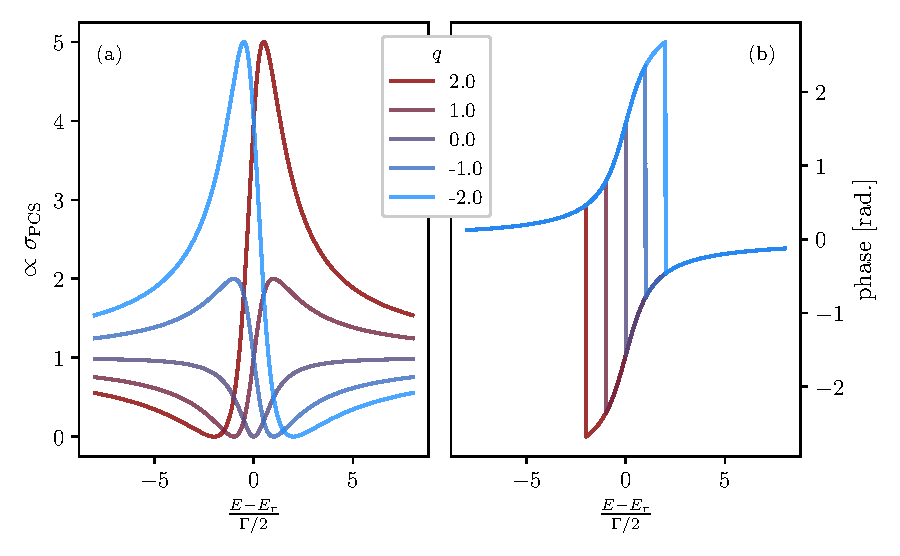
\includegraphics[width=0.8\textwidth]{figures/ATS/cs_phase.pdf}
	\caption[Photoabsorption cross section and phase of a Fano resonance]{(a) Calculation of the photoabsorption cross section near a resonance for the listed $q$ parameters.  The change from symmetric to asymmetric profiles can be seen as the $q$ parameter is varied. Maximum and minimum in cross section occus at $\epsilon=1/q$ and $\epsilon=-q\Gamma^2/4$, respectively. (b) Calculation of the phase across the resonance for different $q$ parameter. The $\pi$ phase jump clearly depends on $q$, and it occurs when $\epsilon=-q$ and not at the resonance energy $E_r$. Calculations based on U. Fano's original work \cite{fanoEffectsConfigurationInteraction1961}.}
	\label{fig:cross_sec_and_phase}
\end{figure}

Experimentally the photoabsorption cross section is generally fit to the form
\begin{equation}
\label{eqn:sigma_pcs}
	\sigma_\mathrm{PCS}=\sigma_a\frac{(q+\epsilon)^2}{\epsilon^2+1}+\sigma_{NR}
\end{equation}
where $\sigma_a$ scales the strength of the Fano profile and $\sigma_{NR}$ is  a non-resonant cross section that is included to account for absorption from  other continuum states that might be present.  



\subsection{Autoionization in the time domain}
\label{sec:time_dependent_autoionization}
%
%!!!!!!!!!!!!!!!!!!!!!!!!!!!!!!!!!!!!!!!!!!!!!!!!!!!!!!!!!!!!!!!!!!!!!!!!!!!!!!!!!
%!!!!!!!!!!!!!!!!!!!!!!!!!!! ATOMIC UNITS !!!!!!!!!!!!!!!!!!!!!!!!!!!!!!!!!!!!!!!!
%!!!!!!!!!!!!!!!!!!!!!!!!!!!!!!!!!!!!!!!!!!!!!!!!!!!!!!!!!!!!!!!!!!!!!!!!!!!!!!!!!
%

Up until this point, Fano resonances have been discussed in a time-independent manner in the frequency domain.  However, one would ideally like to describe these autoionizing resonances in the time domain, as that will lend itself to the experiments described herein. This description was primarily done by W.-C. Chu and C.D. Lin \cite{chuTheoryUltrafastAutoionization2010}, and it has been used to interpret many ATS experiments  \cite{kaldunExtractingPhaseAmplitude2014,ottLorentzMeetsFano2013,ottReconstructionControlTimedependent2014, stoossRealTimeReconstructionStrongFieldDriven2018}.  The basic assumption that is made in this treatment is that the XUV pulse that excites from the ground state to the Fano resonance is a Dirac-$\delta$ function in time, $\mathbf{E}_{XUV}=E_0\delta(t)\mathbf{z}$.  This impulsive excitation is generally a reasonable  approximation for an attosecond XUV pulse that is shorter in duration than the typical lifetimes of these resonances.  From this assumption, it is possible to analytically describe the dipole response of the system in the time domain.


The derivation of the dipole response follows naturally from the theory described in the previous section. Assuming that the XUV impulsively excites at $t=0$ from the ground state $\ket{g}$ to the bound and continuum states $\ket{\psi_b}$ and $\ket{\psi_\varepsilon}$, the wave function for times $t>0$ can be in the configuration states, such that
\begin{equation}
\label{eqn:wvfnc_expansion}
	\ket{\Psi(t)}=e^{-i\varepsilon_gt}\ket{g}+c_b(t)\ket{\psi_b}+\int c_\varepsilon(t)\ket{\psi_\varepsilon}\diff \varepsilon.
\end{equation}
Since the configuration states $\ket{\psi_b}$ and $\ket{\psi_\varepsilon}$ are not eigenstates of the total Hamiltonian, the expansion coefficients $c_b$ and $c_\varepsilon$ are explicitly time dependent. The evolution of these coefficients is governed by the Time-Dependent Schr{\"o}dinger Equation (TDSE)
\begin{equation}
\label{eqn:tdse}
	i\frac{\partial}{\partial t}\ket{\Psi(t)}=\hat{H}\ket{\Psi(t)},
\end{equation}
and using this equation, the time dependence of the expansion coefficients can be expressed as the coupled differential equations given by
\begin{equation}
\label{eqn:coupled_pde}
	\begin{aligned}
		\frac{\partial c_{\varepsilon}}{\partial t} &= -iV_\varepsilon c_b(t)-i\varepsilon c_\varepsilon(t)\\
		\frac{\partial c_b}{\partial t} &= -i\varepsilon_r c_b(t)-iV_\varepsilon \int c_\varepsilon(t) \diff \varepsilon.
	\end{aligned}
\end{equation}
Assuming the initial values $c_b^{(0)}$ and $c_\varepsilon^{(0)}$ are known, then the solutions to equations \ref{eqn:coupled_pde} are given by
\begin{equation}
\label{eqn:coefficients}
	\begin{aligned}
		c_b(t) &= c_b^{(0)}\bigg(1-\frac{i}{q}\bigg)e^{-i\varepsilon_r}e^{-\frac{\Gamma}{2}t}\\
		c_\varepsilon(t) &= \frac{c_\varepsilon^{(0)}}{\epsilon + i}e^{-i\varepsilon_r t}\bigg[ (q+\epsilon)e^{-i(\varepsilon-\varepsilon_r)t}-(q-i)e^{-\frac{\Gamma}{2}t}\bigg],
	\end{aligned}
\end{equation}
where, as in the previous section, $q=c_b^{(0)}/(\pi V c_\varepsilon^{(0)})$, $\Gamma=2\pi\rvert V \lvert^2$, and $\epsilon=(\varepsilon-\varepsilon_r)/(\Gamma/2)$. 


\begin{figure}
	\centering
	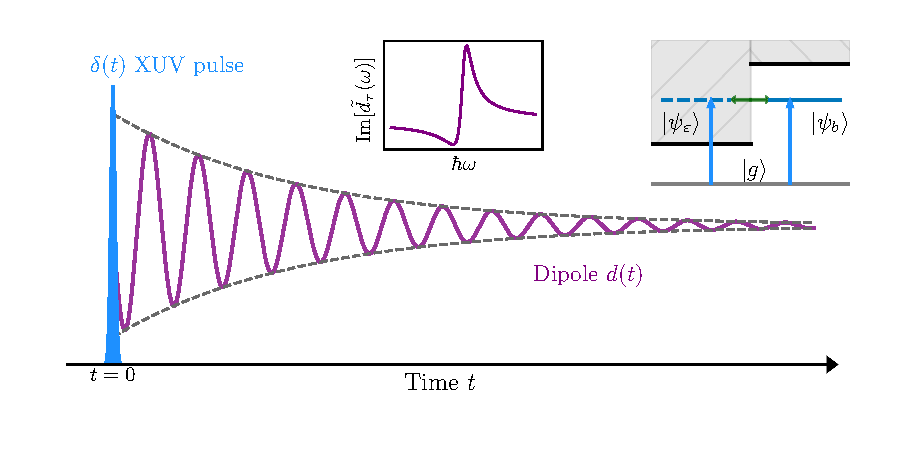
\includegraphics[width=1.0\textwidth]{figures/ATS/dipole_sketch.pdf}
	\caption[Illustration of dipole moment in the time-domain with various phase shifts]{Illustration of the dipole moment after a $\delta(t)$ excitation pulse. Dipole is shown for a phase shift of $\varphi=-1.2\pi$ (purple curve) and $\varphi=0$ (dashed gray curve), and the central inset shows the line shape for these two phase shifts.}
	\label{fig:dipole_sketch}
\end{figure}

With the time dependent wave function now in hand, the induced dipole $d(t)$ can now be calculated for $t>0$ by evaluating  $d(t)=\braket{\Psi(t)|z|\Psi(t)}$.  Using equations \ref{eqn:wvfnc_expansion} and \ref{eqn:coefficients}, this gives
\begin{equation}
\label{eqn:dip}
	\begin{aligned}
		d(t)&=c_b(t)e^{-i\varepsilon_g t}\braket{\psi_b|z|g}^* + \int c_\varepsilon(t)e^{i\varepsilon_g t}\braket{\psi_\varepsilon|z|g}^* + c.c.\\
		&=c_b^{(0)}\braket{\psi_b|z|g}^*e^{-i\Omega_r t}\Bigg[\bigg(1-\frac{i}{q}\bigg)e^{-\frac{\Gamma}{2}t}+ \frac{1}{(\pi V q)^2}\int \frac{(q+\epsilon)e^{-i\frac{\Gamma}{2}\epsilon t}-(q-i)e^{\frac{\Gamma}{2}t}}{\epsilon+i}\diff\varepsilon\Bigg] + c.c.,
	\end{aligned}
\end{equation}
where $\Omega_r=E_r-E_g$ is the resonance photon energy.  The complex conjugate term in equation \ref{eqn:dip} is a counter-rotating term, and by invoking the rotating wave approximation, it can be dropped.  Equation \ref{eqn:dip} can further be evaluated to give
\begin{equation}
	\begin{aligned}
	d(t) &= c_b^{(0)}\braket{\psi_b|z|g}^*e^{-i\Omega_r t}\frac{1}{q^2}\Bigg[q(q-i)e^{-\frac{\Gamma}{2}t}+\frac{2}{\pi\Gamma}\int \frac{(q+\epsilon)e^{-i\frac{\Gamma}{2}\epsilon t}-(q-i)e^{\frac{\Gamma}{2}t}}{\epsilon+i}\diff\varepsilon\Bigg]\\
	&= c_b^{(0)}\braket{\psi_b|z|g}^*e^{-i\Omega_r t}\frac{1}{q^2}\Bigg[q(q-i)e^{-\frac{\Gamma}{2}t} + \frac{1}{\pi} \int e^{-i\frac{\Gamma}{2}\epsilon t}\diff\epsilon + \frac{q-i}{\pi}\int \frac{e^{-i\frac{\Gamma}{2}\epsilon t} - e^{-\frac{\Gamma}{2}t}}{\epsilon+i} \diff\epsilon\Bigg]\\
	&=c_b^{(0)}\braket{\psi_b|z|g}^*e^{-i\Omega_r t}\frac{1}{q^2} \Bigg[ q(q-i)e^{-\frac{\Gamma}{2}t}+ \frac{4}{\Gamma}\delta(t) + \frac{q-i}{\pi}e^{-\frac{\Gamma}{2}t}2\pi i + \frac{q-i}{\pi}e^{-\frac{\Gamma}{2}t}\pi i \Bigg]\\
	&=c_b^{(0)}\braket{\psi_b|z|g}^*\frac{1}{q^2}\bigg[ \frac{4}{\Gamma}\delta(t)+(q-i)^2e^{-i\Omega_r t}e^{-\frac{\Gamma}{2}t}\bigg].
	\end{aligned}
\end{equation}
If we assume that $\braket{\psi_b|z|g}$ is real and the expansion coefficient is $c_b^{(0)}$ purely imaginary, then we can finally arrive at the form of the dipole that is reported in \cite{chuTheoryUltrafastAutoionization2010,ottLorentzMeetsFano2013,kaldunFanoResonancesTime2014},
\begin{equation}
\label{eqn:dipole_time_domain}
	d(t)\propto i\bigg[ 2\delta(t) + \frac{\Gamma}{2}(q-i)^2 e^{-i\Omega_r t}e^{\frac{\Gamma}{2}t} \bigg].
\end{equation}
This form of the dipole can be understood intuitively as arising naturally from the two interfering processes that are occurring: direct ionization to the continuum and decay from a discrete state to the continuum with a lifetime of $\hbar/\Gamma$.  The first $\delta$-function in equation \ref{eqn:dipole_time_domain} represents direct ionization, and the second term represents decay from the discrete state.  A schematic of the dipole after an impulsive XUV pulse is shown in  figure \ref{fig:dipole_sketch}.  To demonstrate that this formulation of the dipole in the time domain is compatible with Fano's original derivation, the photoabsorption cross section can be evaluated by
\begin{equation}
\begin{aligned}
	\sigma&=\frac{2\omega}{\epsilon_0 c}\mathrm{Im}\bigg[\frac{\tilde{d}(\omega)}{\tilde{E}(\omega)}\bigg]\propto \mathrm{Im}\bigg[\int_{-\infty}^{\infty} d(t) e^{i\omega t} \diff t\bigg]\\
	&\propto\mathrm{Re}\bigg[1+\frac{\Gamma}{2}(q-i)^2\int_0^\infty e^{-\frac{\Gamma}{2}t}e^{i(\omega-\Omega_r)t}\bigg]\\
	&\propto\mathrm{Re}\bigg[1 + \frac{(q-i)^2}{1-i\epsilon}\bigg]\\
	& \propto \frac{(q+\epsilon)^2}{\epsilon^2 +1}.
\end{aligned}
\end{equation}
This is exactly the cross section in equation \ref{eqn:sigma_pcs} that was derived previously.

\begin{figure}
	\centering
	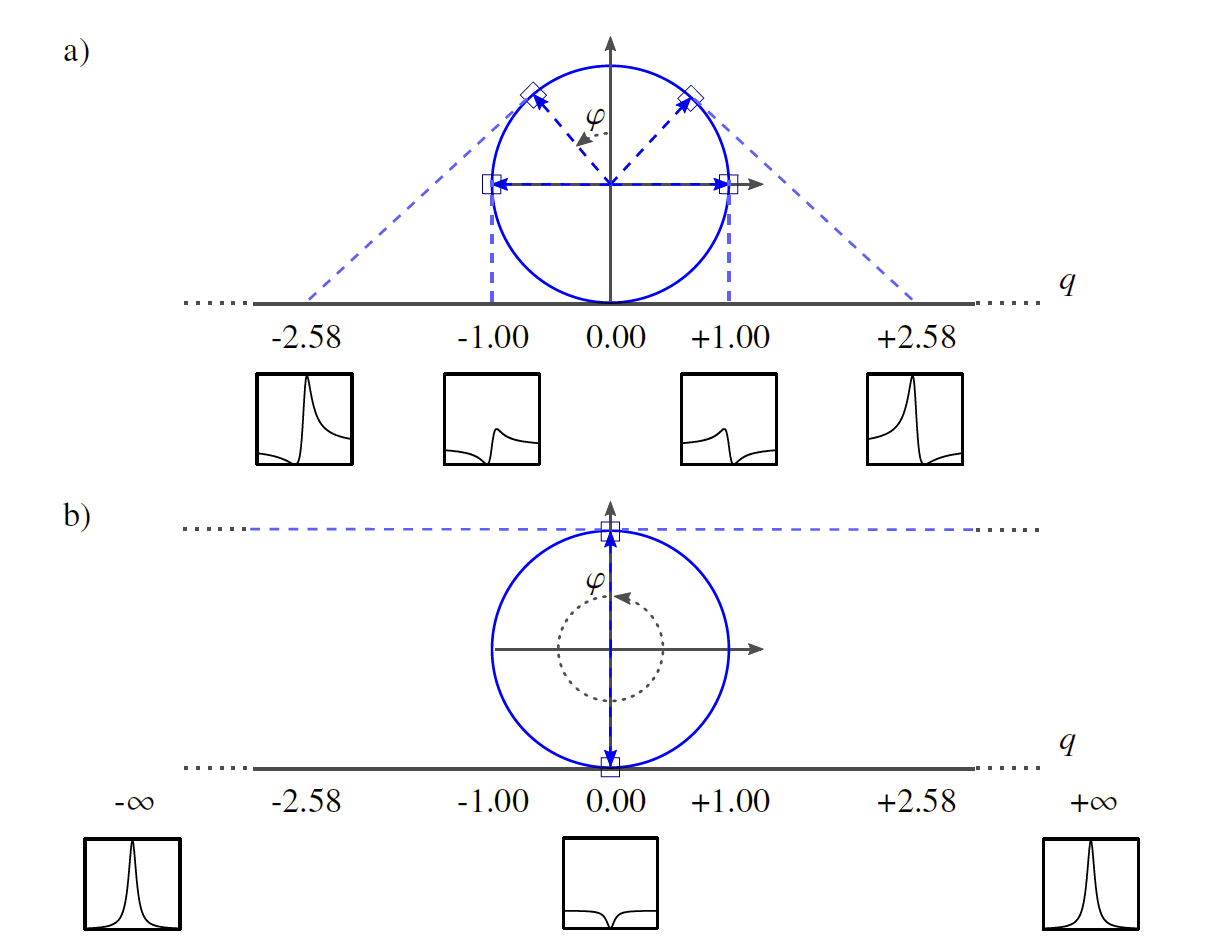
\includegraphics[width=0.8\textwidth]{figures/ATS/Kaldun.png}
	\caption[Illustration of the mapping between the $q-$parameter and the phase shift of the dipole]{Illustration of the mapping between the Fano $q$ parameter and the phase shift $\varphi$ of the dipole. (a) Phase shift $\varphi$ is shown as a counter-clockwise rotation of a vector on the unit circle. Dashed tangent lines for a given $\varphi$ show the mapping to the value $q(\varphi)$ along the $q$-axis. (b) Shows the special cases of a Lorentzian line shape ($q\rightarrow\pm\infty$, $\varphi=0$) and a window resonance ($q=0$, $\varphi=\pi$).  Adapted from \cite{kaldunFanoResonancesTime2014}.}
	\label{fig:q_to_phi}
\end{figure}

The complex coefficient in front of the second term of equation \ref{eqn:dipole_time_domain} arises from the configuration interaction, and its influence on the dipole can be elucidated by expressing it as an exponential,
\begin{equation}
	(q-i)^2 = (q^2+1)e^{i\varphi(q)}
\end{equation} 
where the phase is given by
\begin{equation}
\label{eqn:q-to-phase}
	\varphi(q)=2\arg(q-i).
\end{equation}
Substituting this form into the dipole in equation \ref{eqn:dipole_time_domain} gives
\begin{equation}
\label{eqn:dipole_time_domain_phasse_shift}
	d(t)\propto i\bigg[ 2\delta(t) + \frac{\Gamma}{2}(q^2+1)e^{i\varphi(q)}e^{-i\Omega_r t}e^{\frac{\Gamma}{2}t} \bigg].
\end{equation}
By expressing the dipole this way, it is clear that the autoionization from the discrete state is phase shifted relative to the instantaneous response (direct ionization).  Furthermore, in section \ref{sec:og_fano} it was established that the $q$ parameter determines the line shape of the photoabsorption cross section ($\sigma\propto\mathrm{Im}[\tilde{d}(\omega)]$). This fact, combined with the correspondence between $\varphi$ and $q$, means that the line shape of the Fano resonance is determined by the phase shift of the dipole response.  Thus, if one can experimentally introduce a phase shift of the dipole response then it is possible to control the absorption process.  In fact, if one has sufficient control over the dipole phase shift then it is possible to continuously change the line shape from symmetric to asymmetric and vice versa.  This mapping of $q$ parameter and the phase shift $\varphi$ and its affect on the line shape is shown in figure \ref{fig:q_to_phi}.


\section{Dipole Control Model}
\label{sec:DCM}

Now that the relationship between the dipole and the absorption line shape has been established in the time domain, we would like to establish a method to control and modify the dipole.  This will be done by introducing an IR probe/dressing pulse at a variable time delay $\tau$.  This IR pulse will lead to a modification of the dipole that can be modeled analytically for certain assumptions. This model is referred to as the dipole control model (DCM), and it was originally formulated by A. Bl{\"a}tterman, et al \cite{blattermannImpulsiveControlAtomic2016, blattermannTwodimensionalSpectralInterpretation2014, kaldunFanoResonancesTime2014}. In a similar manner to the previous section, a key assumption that must be made in this model is that, in addition to the XUV pulse, the IR pulse must be a $\delta$-function in time.  This is generally only a reasonable approximation if the pulse duration is much shorter than the lifetime $\hbar/\Gamma$.  These assumptions will be questionable for the experiments discussed in this chapter, however this model will allow for an understanding of the features that will be seen in the data shown later.  


A schematic of the physical situation considered for the DCM is shown in figure \ref{fig:dipole_sketch_dressing}.  A XUV pulse at $t=0$ induces a dipole $d(t)$, and an IR pulse perturbs the dipole after a time delay of $\tau$. The $\delta$-function nature of both pulses means that there are three distinct temporal regions to consider.  The first is $t<0$, and in this region, the dipole response is zero because the XUV pulse hasn't yet populated the excited state. For the region between the two pulses, the dipole is allowed to freely evolve in time, as was derived in \ref{eqn:dipole_time_domain_phasse_shift}. Thus, the dipole response here is just simply
\begin{equation}
	d(0<t<\tau)= f_0(t)\propto i\bigg[ c\delta(t) + \frac{\Gamma}{2}(q-i)^2 e^{-i\Omega_r t}e^{\frac{\Gamma}{2}t} \bigg].
\end{equation}
At $t=\tau$, the dressing field will interact with the system through resonant and non-resonant processes which will modify the dipole response.  However, since the dressing field is infinitesimally short in duration, the system will again freely evolve in time for times after $\tau$, but the dressing field is assumed to have modified the dipole amplitude and phase.  Therefore, in the third temporal region of $t>\tau$, the dipole response is given by
\begin{equation}
	d(t>\tau) = A f_0(t)
\end{equation}
where $A$ is the complex perturbation to the dipole response induced by the dressing pulse. By combing the dipole response for the three temporal regions into a single piece-wise function, we arrive at
\begin{equation}
\label{eqn:piecewise_dipole_t}
	d_\tau(t)=
	\begin{cases}
		0 & t<0\\
		f_0(t) & 0<t<\tau\\
		A(\tau)f_0(t) & t>\tau.
	\end{cases}
\end{equation}

In general, $A$ is a complex quantity that can be explicitly dependent upon $\tau$ or $\omega$, and it can  be used to describe both resonant and non-resonant processes.  For example, a decrease of the amplitude of $A$ can be used to represent ionization of the excited state by the dressing field, whereas the phase can be used to describe a ponderomotive shift of energy levels by the dressing field.  To describe these non-resonant processes, it can be assumed that $A$ takes the form of $A=a_1e^{i\phi_1}$.  To describe a resonant process such as coupling of excited states, $A$ takes the form $A=1+a_2e^{i(\Delta\omega\tau+\phi_2)}$ where $\hbar\omega$ is the separation of the states.  This form is motivated by the results of perturbation theory (see appendix \ref{chap:Perturbation_theory}).  These two primitive forms can be linearly combined into
\begin{equation}
	A=a_1e^{i\phi_1}(1+a_2e^{i(\Delta\omega\tau+\phi_2)}).
\end{equation}
All of these quantities can be explicitly dependent upon $\tau$ and $\omega$, however they are independent of $t$ given the $\delta$-function pulse durations that are assumed. An illustration of these processes is shown in the level diagram in figure \ref{fig:level_diagram_dressing}.

\begin{figure}
	\centering
	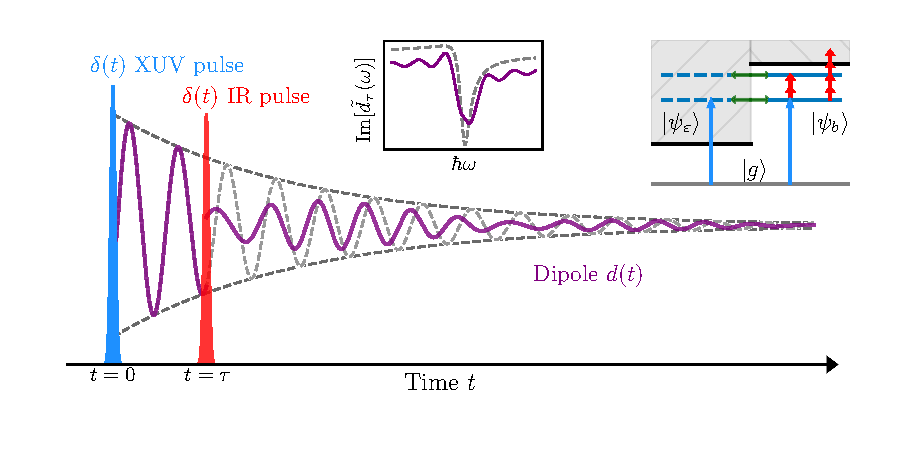
\includegraphics[width=1.0\textwidth]{figures/ATS/dipole_sketch_dressing.pdf}
	\caption[Illustration of the dipole response after being modified by an IR dressing pulse]{Illustration of the dipole response being modified by an impulsive IR pulse.  The IR pulse is shown to arrive after a time delay $\tau$.  The dipole is allowed to freely evolve between $t=0$ and $t=\tau$, but after the IR pulse it is modified in amplitude and phase.  The effect that this has on the absorption cross section is shown in the central inset for a time delay immediately after $\tau$.  Inset on the upper right shows both non-resonant and resonant processes that can be induced with the IR pulse.}
	\label{fig:dipole_sketch_dressing}
\end{figure}

Armed with the dipole in the time domain, it is now possible to calculate the photoabsorption cross section that is the typical observable in a ATS experiment.  To do this, one must calculate the spectral dipole in the frequency domain, and this is done by simply Fourier transforming the dipole in equation \ref{eqn:piecewise_dipole_t},
\begin{equation}
	\begin{aligned}
	\tilde{d}_\tau(\omega,\tau)&=\int_{-\infty}^{\infty} d_\tau(t,\tau)e^{i\omega t}\diff t\\
	&=\int_0^\tau f_0(t)e^{i\omega t}\diff t + \int_\tau^\infty A(\tau)f_0(t)e^{i\omega t}\diff t\\
	&=\int_0^\tau i\bigg[ 2\delta(t) + \frac{\Gamma}{2}(q-i)^2 e^{-i\Omega_r t}e^{\frac{\Gamma}{2}t} \bigg]e^{i\omega t}\diff t \\ & + A(\tau)\int_\tau^\infty i\bigg[ 2\delta(t) + \frac{\Gamma}{2}(q-i)^2 e^{-i\Omega_r t}e^{\frac{\Gamma}{2}t} \bigg]e^{i\omega t}\diff t\\
	&=i-\gamma(q-i)^2\frac{1-(1-A(\tau))e^{-\gamma\tau +i\delta\tau}}{\delta+i\gamma}
	\end{aligned}
\end{equation}
where $\gamma = \Gamma/2$ and $\delta=\omega-\omega_r$.  The photoabsorption cross section is now given by
\begin{equation}
\label{eqn:sigma_pcs_dcm}
	\begin{aligned}
	\sigma(\omega,\tau)&=\frac{2\omega}{\epsilon_0 c}\mathrm{Im}\bigg[\frac{\tilde{d}(\omega)}{\tilde{E}(\omega)}\bigg]\propto \mathrm{Im}\bigg[\int_{-\infty}^{\infty} d(t) e^{i\omega t} \diff t\bigg]\\
	&\propto \mathrm{Im}\bigg[i-\gamma(q-i)^2\frac{1-(1-A(\tau))e^{-\gamma\tau +i\delta\tau}}{\delta+i\gamma}\bigg]\\
	&= \frac{(q+\delta/\gamma)^2}{(\delta/\gamma)+1} + \mathrm{Im}\bigg[\frac{\gamma(q-i)^2(1-A(\tau))e^{-\gamma\tau +i\delta\tau}}{\delta+i\gamma}\bigg].
	\end{aligned}
\end{equation} 
From this, we can now begin to see the effect that of dressing pulse can have on the cross section.  For the case of $A(\tau)=1$, the second term in equation \ref{eqn:sigma_pcs_dcm} goes to zero, and only the unperturbed cross section represented by the first term remains.\footnote{This can be seen by noting that $\epsilon=\delta/\gamma$.}  This is expected because $A(\tau)=1$ implies that there is no interaction between the dressing field and the system.  For the more interesting case of $A(\tau)\neq1$, the dipole and the cross section will be modulated as a function of both photon energy $\omega$ and time delay $\tau$.  The specific functional form of $A(\tau)$ will ultimately determine the line shape, and a couple of cases will be discussed herein.  It is important to note that as $\tau\rightarrow\infty$, the cross section returns to the unperturbed case. This due to the fact that the dipole is allowed to freely evolve over the natural lifetime of the state $\hbar/\Gamma$ before the dressing pulse arrives.

\begin{figure}
	\centering
	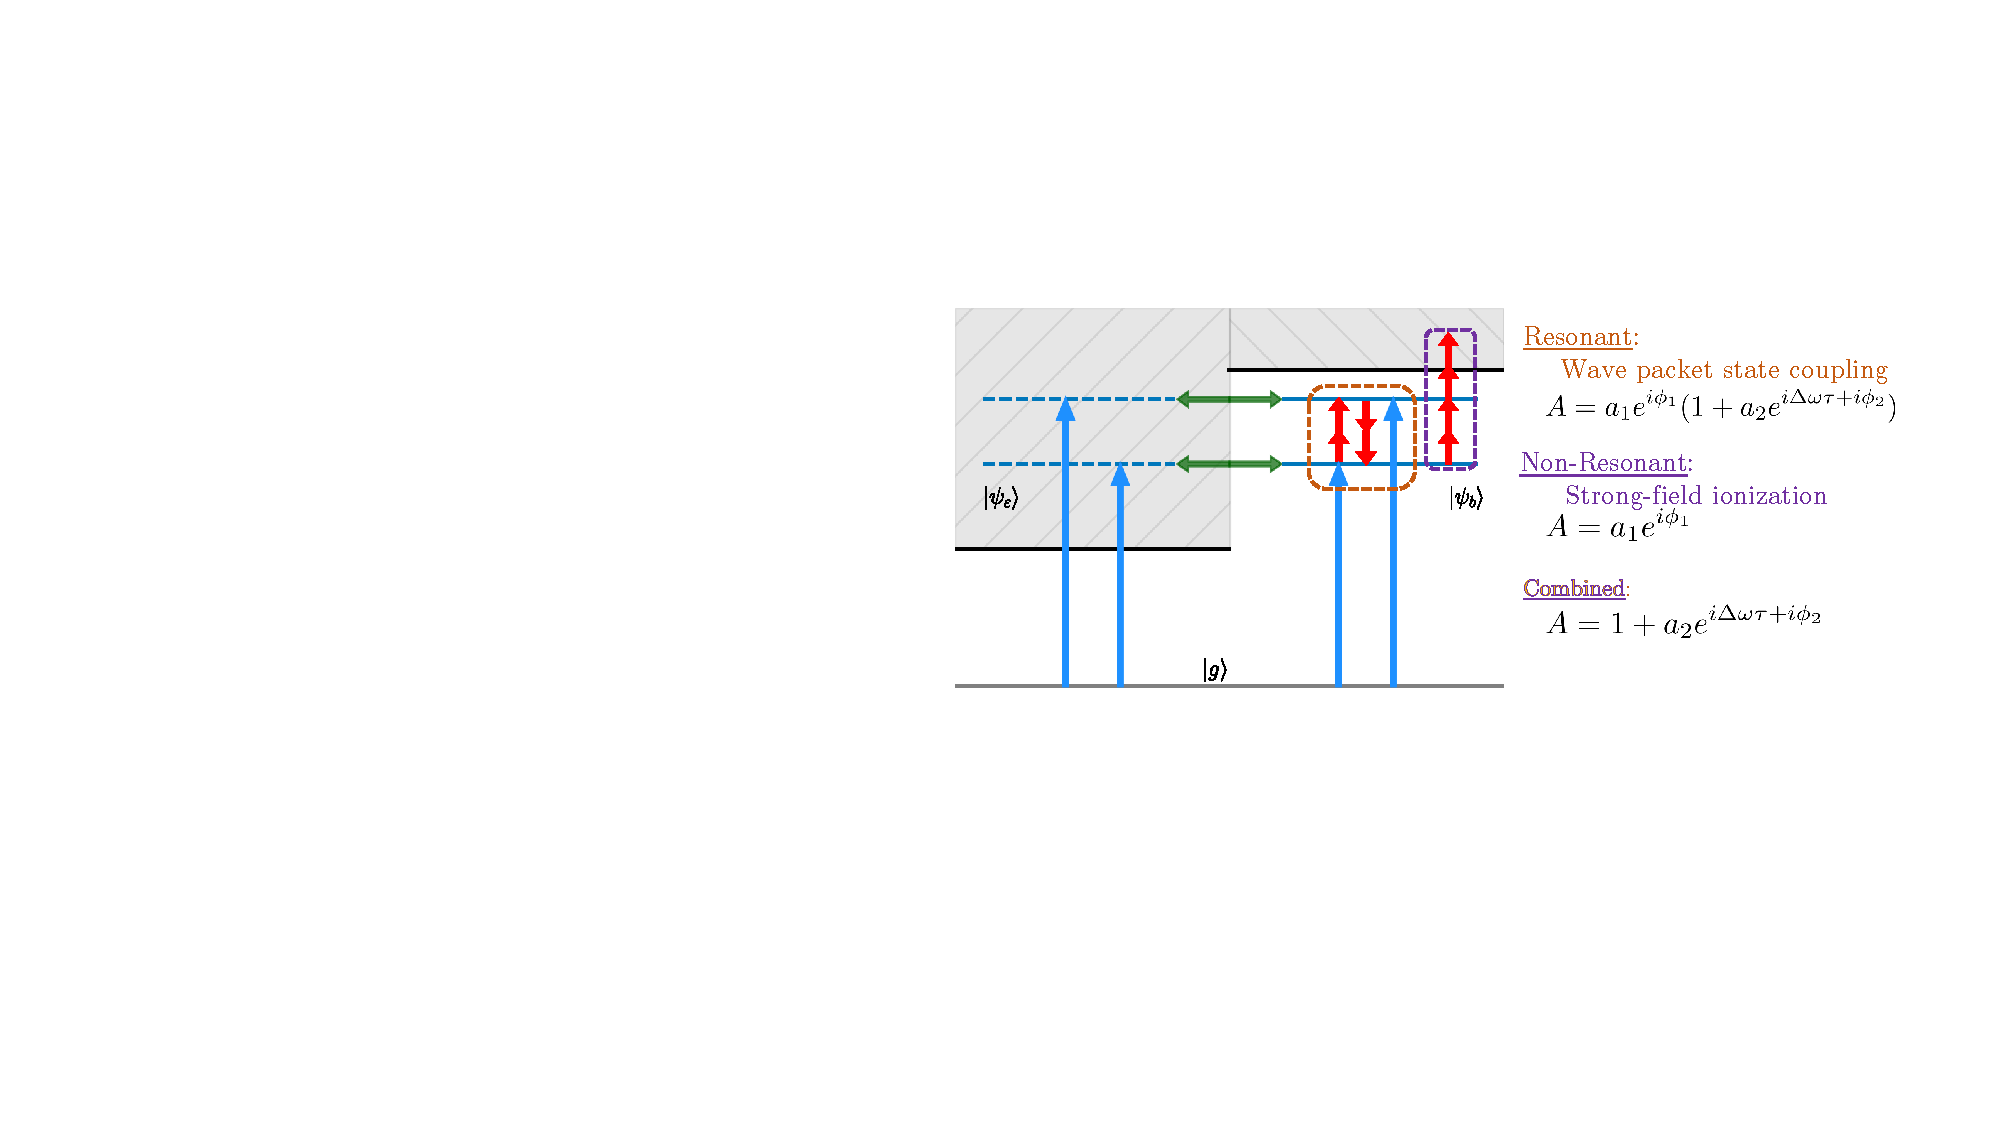
\includegraphics[width=0.8\textwidth]{figures/ATS/level_diagram_dressing_3.pdf}
	\caption[Level diagram showing the influence of the IR dressing pulse on a series of Fano resonances]{Level diagram showing the influence of the IR dressing pulse on a series of Fano resonances. Generally, the IR field can either couple different resonances or directly ionize from the discrete state. Coupling is shown here as a two-photon transition between discrete states, and direct ionization from a discrete state is shown as a multiphoton process.  Green arrows represent the configuration interaction coupling the discrete states to the continuum.}
	\label{fig:level_diagram_dressing}
\end{figure}

In general, there are two primary cases to consider: resonant and non-resonant processes. For a non-resonant process, it can be assumed that the $A(\tau)=a_1e^{i\phi_1}$, and the cross section is plotted in figure \ref{fig:res_vs_non_res}(a) assuming the extreme case of $a_1=\phi_1=0$.  This assumption corresponds to complete ionization of the discrete state by the dressing pulse, and correspondingly, the dipole is quenched for $t>\tau$.  Even this extremely simple model is able to reproduce the common hyperbolic features that occur for $\delta\tau=\mathrm{const.}$ and have been observed in many transient absorption experiments \cite{wangAttosecondTimeResolvedAutoionization2010, ottReconstructionControlTimedependent2014, kaldunObservingUltrafastBuildup2016, wuTheoryStrongfieldAttosecond2016}.  These hyperbolic features arise as a physical manifestation of the ringing described by Gibb's phenomenon which occurs because the observable in the measurement (the cross section) is the Fourier transform of a truncated signal (the dipole) \cite{liInvestigationCouplingMechanisms2015, gibbsFourierSeries1898}. The other dominant feature that can be seen in figure  \ref{fig:res_vs_non_res}(a) is a broadening of the resonance width for $t<\hbar/\Gamma$ that is due to the abrupt quenching of the dipole before it is allowed to freely develop over the state's lifetime.  The spectral width for this region is proportional to $1/\tau$, and it asymptotically approaches the natural width for $\tau\rightarrow\infty$.

\begin{figure}
	\centering
	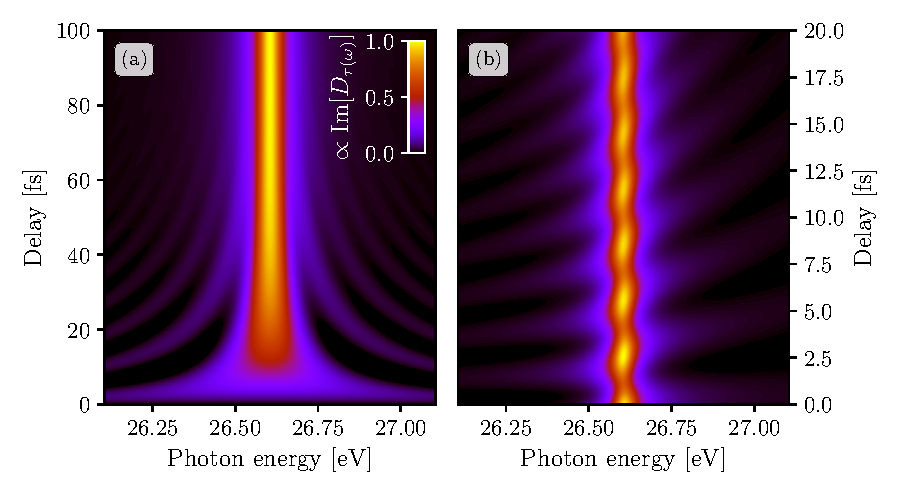
\includegraphics[width=1.0\textwidth]{figures/ATS/resonant_vs_non_resonant.pdf}
	\caption[Imaginary part of the dipole for resonant and non-resonant effects introduced by dressing field]{Imaginary part of the dipole plotted as a function of photon energy and delay. Resonance position is taken to be 26.605 eV, and the line shape is Lorentzian ($\varphi$=0).  (a) Non-resonant case showing complete ionization by dressing field: $a_1=1$ and $\phi_{1}=0$.  (b) Resonant case showing coupling between states: $a_2=0.1$, $\phi_{2}=\pi/4$, and  $\hbar\Delta\omega=1.39$ eV.}
	\label{fig:res_vs_non_res}
\end{figure}

For a resonant process, it can be assumed that $A(\tau)=1+a_2e^{\Delta\omega\tau + i\phi_2}$, and the cross section for such a process is plotted in figure \ref{fig:res_vs_non_res}(b) assuming that $a_2=0.1$, $\phi_2=\pi$, and $\hbar\Delta\omega = 1.39$ eV.  This form of $A(\tau)$ is motivated by time-dependent perturbation theory, and it can be used to describe coupling of states in a wave packet \cite{blattermannImpulsiveControlAtomic2016, blattermannTwodimensionalSpectralInterpretation2014, ottReconstructionControlTimedependent2014, kaldunFanoResonancesTime2014}.  The idea is that the XUV pulse coherently excites a wave packet of multiple excited states, and then the dressing field couples states through multiphoton transitions. This coupling leads to an oscillation in the cross section's amplitude as a function of delay that is the result of a quantum path interference.  This interference can be clearly seen in \ref{fig:res_vs_non_res}(b) with a frequency of $\hbar\Delta\omega=1.39$ eV at the resonance energy.  An additional feature that is present in \ref{fig:res_vs_non_res}(b) is a tilting of the oscillation pattern.  This effect arises because the transition frequency is varying across the resonance as a function of photon energy due to the term $e^{i(\delta+\Delta\omega)\tau}$ in equation \ref{eqn:sigma_pcs_dcm} with the resonant form of $A(\tau)$.  It is important to emphasize that this description only applies to coupling of states that have been coherently excited because the quantum path interference that gives rise to this oscillation requires a common clock between the coupled states.  This is not the case for the dressing field coupling a bright state (one that is initially populated) to a dark state (one that is initially unpopulated).  This dark state coupling will only appear as a depletion of the bright state population and is similar to the non-resonant case described previously.

The importance of this simple analytical model is that it allows for an intuitive description of features that will be seen in the ATS experiment that will be described later in this chapter.  Additionally, the full complex dipole can be calculated with this model, not just the typical observable that is the cross section ($\propto\mathrm{Im}[\tilde{d}(\omega)]$).  This will be used to describe the results in chapter \ref{chap:CATS} where the full complex dipole will be measured.  The complex parts, amplitude, and phase for the non-resonant and resonant cases described above are plotted in  figure \ref{fig:dip_components}.

\begin{figure}
	\centering
	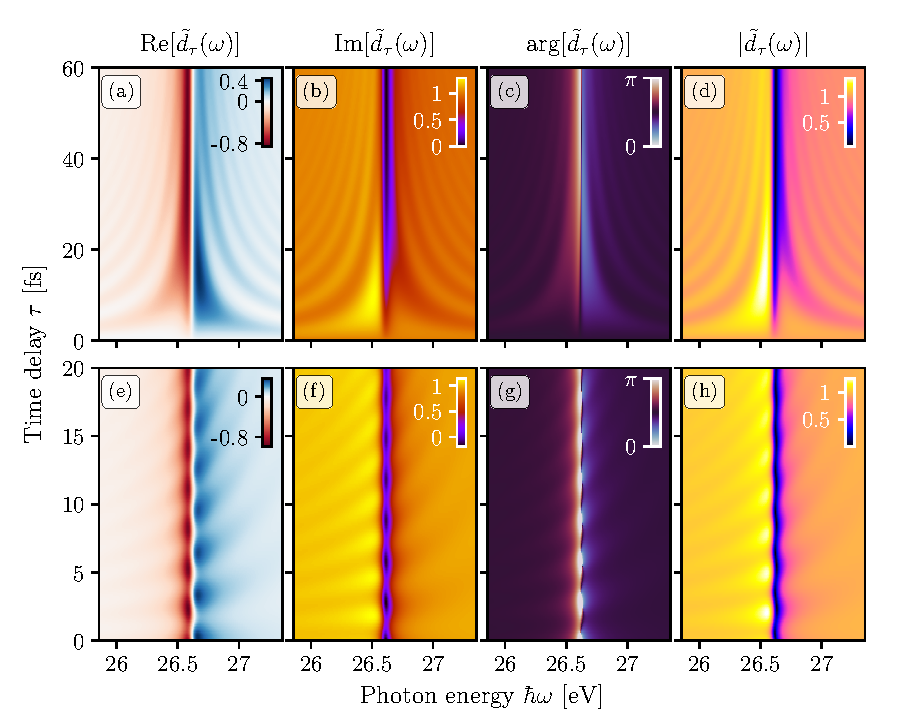
\includegraphics[width=1.0\textwidth]{figures/ATS/dipole_components.pdf}
	\caption[Complex parts, phase, and amplitude of $\tilde{d}_\tau(\omega)$ calculated for resonant and non-resonant interactions]{Complex parts, phase, and amplitude of $\tilde{d}_\tau(\omega)$ calculated for non-resonant ((a) - (d)) and resonant ((e) - (h)) cases for a resonance at 26.605 eV with $q=-0.258$. Parameters for $A(\tau)$ are $a_1=1$ and $\varphi_1=0$ for non-resonate and $a_2=0.1$, $\phi_2=\pi/4$, and $\hbar\Delta\omega=1.39$ eV for resonant.}
	\label{fig:dip_components}
\end{figure}

Further insight into these resonant and non-resonant mechanisms can be gained by Fourier transforming along the time delay axis and examining the characteristic frequencies associated with each process.  Specifically, the typical observable (the cross section) is Fourier transformed and this expression is given by
\begin{equation}
\label{eqn:2DAS_fourier_transform}
	\tilde{d}_\nu(\omega, \nu)=\int_{-\infty}^{\infty}\mathrm{Im}[\tilde{d}_\tau(\omega, \tau)]e^{-i\nu\tau}\diff\tau\propto\int_{-\infty}^{\infty}\sigma(\omega, \tau)e^{-i\nu\tau}\diff\tau.
\end{equation}  
Effectively, this represents two Fourier transforms of the time domain dipole: one that physically occurs by measuring the cross section and another that is performed numerically.  This is a two-dimensional spectroscopic representation that will be referred to as the two-dimensional absorption spectrum (2DAS) \cite{blattermannTwodimensionalSpectralInterpretation2014, blattermannImpulsiveControlAtomic2016}. The main advantage of analyzing the absorption spectrogram in this manner is that different physically processes are naturally separated because of their differing frequency response.

To see this more clearly, the two general cases of resonant and non-resonant interactions introduced by the IR dressing field will be considered.  The first process to consider is the non-resonant case that deals with both direct ionization and energy level shifts by the dressing field, as well as modifications of the dipole phase and $q$-parameter.  These effects are generally described by the complex form $A(\tau)=a_1e^{i\phi_1}$, and the 2DAS for two sets of $a_1$ and $\phi_1$ parameters is shown in \ref{fig:non_res_high_low}. The immediately striking feature that appears in $\rvert\tilde{d}_\nu(\omega)\lvert$ are strong lines that original at the resonance photon energy and zero Fourier frequency.  There are three lines in total with a vertical line occurring at the resonance energy $\omega_r$  and two diagonal lines that for $(\omega-\omega_r)\pm\nu=0$. The diagonal lines have a slope of one, and they correspond to the hyperbolic features that occur in the cross section because of truncation of the dipole in the time domain by the dressing field.  The vertical line that occurs at the resonance energy is related to bandwidth of the non-resonant process.  Since the dressing field is approximated as an instantaneous change of the dipole, the bandwidth in this case extends over all frequencies, however this won't be the case fo a finite pulse duration for the dressing field.  From the amplitude $\rvert\tilde{d}_\nu(\omega)\lvert$ and phase $\mathrm{arg}[\tilde{d}_\nu(\omega)]$ of these features it is possible to extract both $a_1$ and $\phi_1$ which can characterize the type of non-resonant process that is occurring. 
\begin{figure}
	\centering
	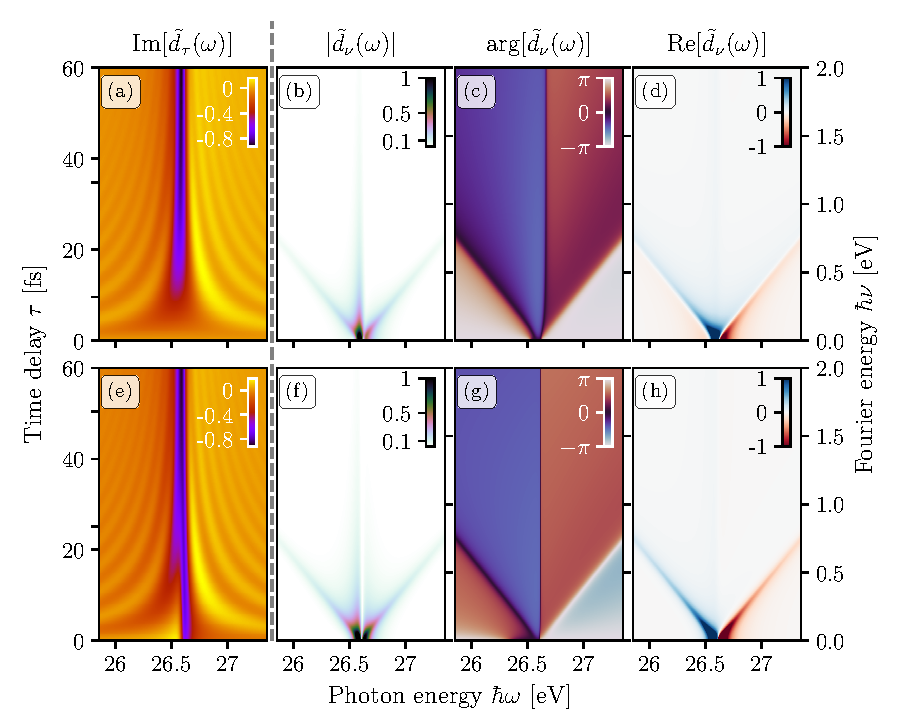
\includegraphics[width=1.0\textwidth]{figures/ATS/DCM_non_res_high_low.pdf}
	\caption[Fourier transform of the dipole, $\tilde{d}_{\nu}(\omega)$, for the non-resonant interaction case]{Fourier transform of the dipole, $\tilde{d}_{\nu}(\omega)$, for the non-resonant interaction case where $A(\tau)=a_1e^{i\phi_1}$.  Resonance  shown here has a resonance energy of 26.605 eV and a $q$-parameter of -0.258.  Figures (a)-(d) are for complete ionization by the dressing field, and this corresponds to $a_1=0,\phi_1=0$.  Figures (e)-(h) are for partial ionization with a phase shift, and this corresponds to $a_1=0.8,\phi_1=\pi/2$.}
	\label{fig:non_res_high_low}
\end{figure}

\begin{figure}
	\centering
	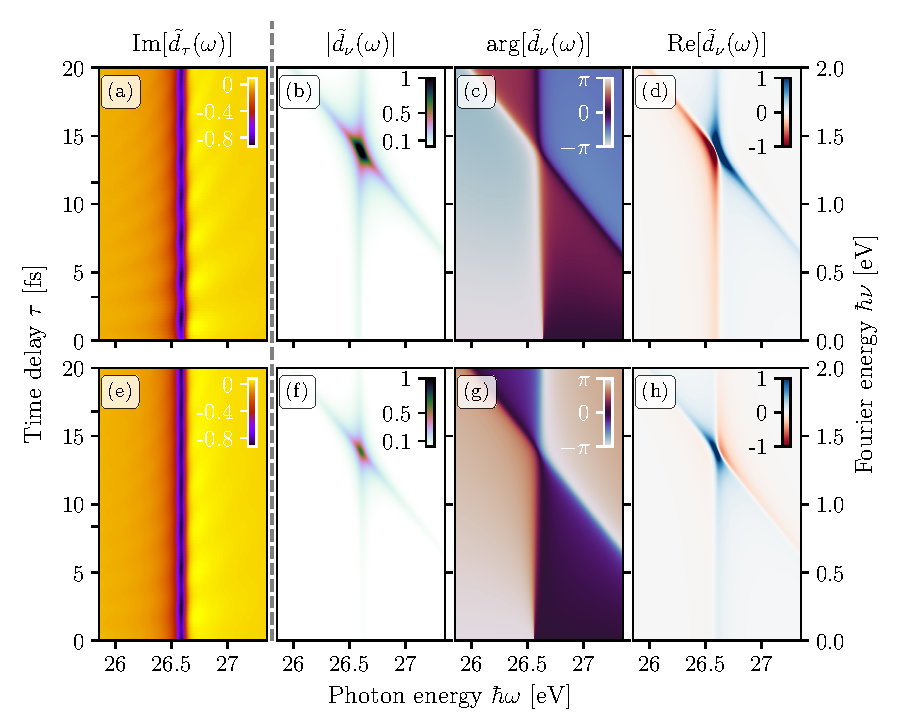
\includegraphics[width=1.0\textwidth]{figures/ATS/DCM_res_high_low.pdf}
	\caption[Fourier transform of the dipole, $\tilde{d}_{\nu}(\omega)$, for the resonant interaction case]{Fourier transform of the dipole, $\tilde{d}_{\nu}(\omega)$, for the resonant interaction case where $A(\tau)=1+a_2e^{i\Delta\omega\tau + i\phi_2}$. Resonance shown here has a resonance energy of 26.605 eV and a $q$-parameter of -0.258.  Figures (a)-(d) are for a coupling strength and phase shift give by $a_2=0.1,\phi_1=\pi$.  Figures (e)-(h) are for a coupling strength and phase shift give by $a_2=0.05,\phi_1=\pi/2$.}
	\label{fig:res_high_low}
\end{figure}

\begin{figure}
	\centering
	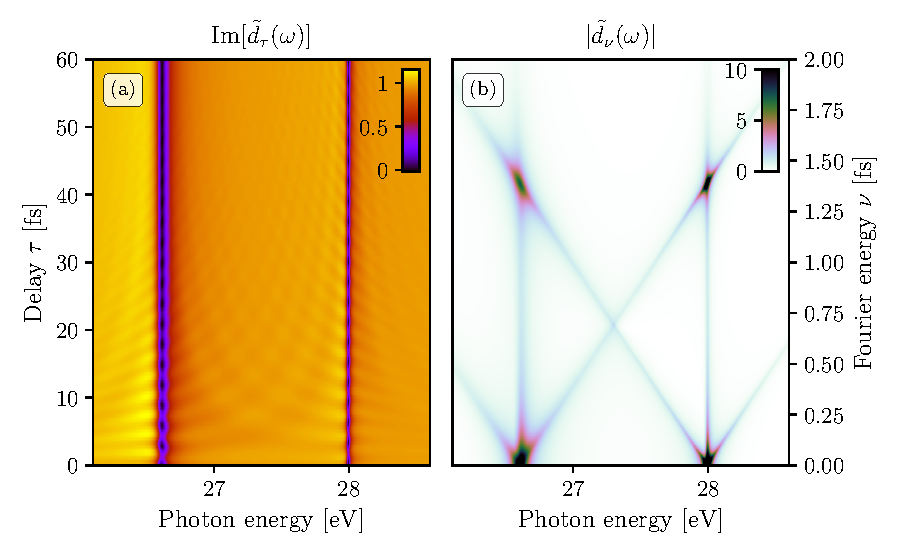
\includegraphics[width=0.9\textwidth]{figures/ATS/multiple_resonances.pdf}
	\caption[Fourier transform of the dipole, $\tilde{d}_{\nu}(\omega)$, for resonant and non-resonant interactions with two resonances]{Fourier transform of the dipole, $\tilde{d}_{\nu}(\omega)$, for resonant and non-resonant interactions with two resonances. $\phi_0=4p$ $a_2=0.1,\phi_2=\pi$, $a_2=0.05,\phi_2=\pi/2$}
	\label{fig:multiple_resonances}
\end{figure}

The other case to consider is resonant interactions introduced by the dressing field.  This usually comes in the form of coupling bright states populated by the XUV pulse, and, by coupling states within a wave packet in this manner, a fast modulation of the cross section will arise.  Within this model, it can be assumed that the form for this type of interaction is given by $A(\tau)=1+a_2e^{i\Delta\omega\tau+i\phi_2}$ where $\Delta\omega$ is the energy separation of the states being coupled and $\phi_2$ is the phase that is imparted. This is shown in figure \ref{fig:res_high_low} for two different coupling strengths and imparted phase shifts.  From the Fourier transform of the delay dependent dipole in figures \ref{fig:res_high_low} (b) and \ref{fig:res_high_low} (f), it can be seen that these modulations occur at a Fourier frequency corresponding to the energy separation of the states being coupled ($\nu=\Delta\omega$).  Also of note are the diagonal structures whose amplitude is center at $(\delta,\nu)=(0,\Delta\omega)$.  The diagonal line is given by $\delta+\Delta\omega\pm\nu=0$, and it effectively "points" to the resonance that is being coupled.  This can be seen most clearly in figure \ref{fig:multiple_resonances} where the two resonances that are being coupled are shown.  Additionally, by looking at the amplitude of the peak at $(\delta,\nu)=(0,\Delta\omega)$ the amplitude of the coupling strength $a_2$ can be determined because this peak is proportional to $a_2$.  The effect of the imparted phase $\phi_2$ can be seen clearly by looking at the phase of the Fourier transform ($\arg[\tilde{d}_{nu}(\omega)]$) in figures \ref{fig:res_high_low} (c) and \ref{fig:res_high_low} (g).  The overall structure between the two cases is the same, but the actual phase shifts across these structures is modified by the phase that is imparted by the dressing field.  From the amplitude $\rvert\tilde{d}_\nu(\omega)\lvert$ and phase $\mathrm{arg}[\tilde{d}_\nu(\omega)]$ of these features it is possible to extract both $a_2$, $\Delta\omega$, and $\phi_2$ which characterizes the resonant interaction.



\subsection{Light-Induced Phase}
\label{sec:LIP}
In the previous section, the parameters that characterized the modification to the dipole in the DCM were kept as general as possible and just treated as a parameter that could be delay dependent.  In this section and the next, specific forms for the non-resonant parameters $\phi_1$ and $a_1$ will be introduced, and this treatment will allow for an extension of the DCM to dressing fields with a finite pulse duration.  This section will discuss the light-induced phase (LIP) whose effect is captured by $\phi_1$. 

In section \ref{sec:time_dependent_autoionization}, the connection between the dipole phase and the absorption lineshape was established through the relationship given in equation \ref{eqn:q-to-phase}.  In the DCM, the natural phase of the resonance is modified by the phase introduced through the parameter $\phi_1$.  Thus, the LIP given by $\phi_1$ controls the absorption lineshape of the bright resonance.  In very general terms, this LIP originates from the energetic Stark shift $\Delta\varepsilon(t,\tau)$ of a bright state that is the result of coupling to nearby states.  This LIP can be generally calculated using the relationship
\begin{equation}
	\label{eqn:LIP}
	\phi_{1}(t,\tau) = \frac{1}{\hbar}\int_{0}^{t}\Delta\varepsilon(t',\tau)\diff t'
\end{equation}
where the assumption is made that the XUV pulse is still delta function in time and populates the bright state at a time $t=0$.\footnote{Otherwise, the integration limits would extend from $-\infty$ to $t$.}  This description of the total accumulated phase allows for dressing pulses that have finite pulse duration.  Thus, the challenge now is to calculate the Stark shift $\Delta\varepsilon(t,\tau)$ for a given system.

There are several models to calculate this energy shift, and three of these will be discussed herein.  The first method is to consider the electron in the bright state as a quasi-free electron that couples very weakly to nearby states and is weakly bound. This assumption means that the energy shift will be related to the ponderomotive energy that the electron picks up from the field.  The energy shift can be calculated classically as
\begin{equation}
	\label{eqn:up_energy_shift}
	\Delta\varepsilon(t,\tau)=\frac{1}{2}m v(t,\tau)^2=\frac{e^2}{2m}\bigg[\int_{-\infty}^{t}\mathcal{E}(t',\tau)\diff t'\bigg]^2
\end{equation}
where $\mathcal{E}(t,\tau)$ is the electric field of the dressing pulse.  This method was used to describe several experiments that were performed in He \cite{ottLorentzMeetsFano2013, blattermannSituCharacterizationFewcycle2015}.

The second method to calculate the energy shift is to use second order time dependent perturbation theory \cite{chiniSubcycleAcStark2012,chiniCharacterizationApplicationIsolated2012,bransdenPhysicsAtomsMolecules2003, griffithsIntroductionQuantumMechanics2005}.  This method is a sub-cycle extension of the optical ac Stark shift, where the energy shift $\Delta\varepsilon_a$ of state a is given by
\begin{equation}
	\label{eqn:optical_stark}
	\Delta\varepsilon_a=-\frac{1}{2}\sum_{k\neq a}\frac{\omega_{ka}\rvert d_{ka} \lvert^2}{\omega_{ka}^2 - \omega_L^2}\langle E(t)^2 \rangle =-\frac{1}{2}\alpha_a \langle E(t)^2 \rangle
\end{equation}
where $\alpha_a$ is the polarizability of state a, $d_{ka}$ is the dipole matrix element between states $a$ and $k$, $\omega_L$ is the dressing frequency, and $E(t)=E_0(t)\cos(\omega_L t)$ is the electric field.  This is an inherently cycle averaged effect, but it can be extended to a sub-cycle ac Stark shift using second order perturbation theory. The energy shift for this case is given by
\begin{equation}
	\label{eqn:SOPT}
	\Delta \varepsilon_a(t,\tau)=-i\sum_{k\neq a}d_{ak}\mathcal{E}(t-\tau)e^{i\omega_{ak}t}\int_{-\infty}^{t} d_{ka}\mathcal{E}(t'-\tau)e^{i\omega_{ka}t}\diff t'.
\end{equation}
For a pulse shape that is given by $\mathcal{E}_0(t)=\mathcal{E}_pe^{-\rvert t \lvert/t_p}$, the integrals can be solved analytically to give
\begin{equation}
	\label{eqn:SOPT_integrated}
	\begin{aligned}
	\Delta\varepsilon_a(t,\tau) &=\frac{1}{2}\mathcal{E}_0(t-\tau)^2\sum_{k\neq a}\bigg[ \frac{\omega_{ka}\rvert d_{ka} \lvert^2}{\omega_{ka}^2 - \omega_L^2}\cos(\omega_L (t-\tau))^2 -i\frac{\omega_{L}\rvert d_{ka} \lvert^2}{\omega_{ka}^2 - \omega_L^2}\sin(2\omega_{L} (t-\tau))\bigg]\\
	&=\frac{1}{2}\mathcal{E}_0(t-\tau)^2[\alpha_a\cos(\omega_{L} (t-\tau))^2 - i\gamma_{a}\sin(2\omega_{L} (t-\tau))].
	\end{aligned}
\end{equation}
where $\alpha_a$ is the polarizability of state $a$ and $\gamma_{a}$ is related to the population change in state a as it is being coupled to state k.  This form for the energy level shift is generally only accurate when the frequency of the dressing field is far from resonance and the peak Rabi frequency $\Omega_{ka} = d_{ka}E_p$ is much less than the energy level separation.

The third method to calculate the energy level shift from the dressing field involves the use of Floquet theory and the rotating-wave approximation (RWA)\cite{wuTheoryStrongfieldAttosecond2016}.  Floquet theory will be discussed in more detail in section \ref{sec:LIS_Floquet} to describe light-induced states, but it will be briefly discussed here as a means to derive the energy shift of a bright state in a simple two-level system consisting of a bright state $\ket{1}$ and a dark state $\ket{2}$ with energies of $\omega_1$ and $\omega_2$ in atomic units.  In the Floquet basis, the wave function can be expanded in such a way that the time evolution of the dressed states is simply a phase gain,
\begin{equation}
	\ket{\psi(t)} = \sum_{\alpha,n}C_{\alpha}e^{-i(\varepsilon_\alpha+n\omega_L)t}\ket{\phi_\alpha,n}.
\end{equation}
where $\ket{\phi_\alpha,n}$ and $C_{\alpha}=\braket{\phi_{\alpha,n}|1}$ are the Floquet states and initial amplitude, respectively.  The amplitude  in the bright state is then given by 
\begin{equation}
	\begin{aligned}
		C_1(t)&=\braket{1|\psi(t)}=\sum_{\alpha,n}\braket{1|\phi_{\alpha,n}}\braket{\phi_{\alpha,n}|1}e^{-i(\varepsilon_\alpha+n\omega_L)t}\\
		&\approx \braket{1|\phi_{+,0}}\braket{\phi_{+,0}|1}e^{-i\varepsilon_{+} t},
	\end{aligned}
\end{equation}
where in the last step the approximation was made that $\braket{\phi_{\alpha,n}|1}\approx0$ except for $\braket{\phi_{+,0}|1}$.  It can be seen from this relation that the Floquet theory naturally agrees with the LIP picture where the bright state is modified only in an accumulation of phase.  Therefore, the energy shift that can be used to calculate the LIP is given by
\begin{equation}
	\Delta\varepsilon=\varepsilon_{+}-\omega_1
\end{equation}
where $\omega_1$ is the energy of the bright state.  Thus, the problem has been reduced to calculating the Floquet energy $\varepsilon_+$.  This calculation can be done using the RWA to calculate the first-order Floquet energy, and this is shown in the review by Wu, et al \cite{wuTheoryStrongfieldAttosecond2016}.  The resulting expression for the Floquet energy is given by
\begin{equation}
	\label{eqn:Floquet_energy_shift}
	\Delta\varepsilon_+ = \omega_1+\frac{-\Delta+\sqrt{\Delta^2+\Omega(t,\tau)^2}}{2},
\end{equation}
where $\Delta=\omega_L-(\omega_2-\omega_1)$ is the detuning of the dressing frequency from resonance and $\Omega(t,\tau)=d_{21}\mathcal{E}(t,\tau)$ is the Rabi frequency.  Thus, the time-dependent energy level shift is given by
\begin{equation}
	\Delta\varepsilon(t,\tau)=\frac{-\Delta+\sqrt{\Delta^2+\Omega(t,\tau)^2}}{2}.
\end{equation}
The advantage of this method to calculate the energy level shift is that it does not require the dressing frequency to be far from resonant, and this method works best when the detuning is small.  This is due to the use of the RWA approximation in this derivation, and it can be generally shown that the RWA is most appropriate when the detuning is small and the dynamics are dominated by Rabi cycling \cite{wuTheoryStrongfieldAttosecond2016,wuTimedomainPerspectiveAutlerTownes2013}.

\subsection{Light-Induced Attenuation}
\label{sec:LIA}
An additional term in the DCM that can be explicitly calculated for a dressing pulse of finite pulse duration is the non-resonant amplitude $a_1$, which,  as stated previously, is related to the population of the discrete state.  For typical experimental conditions that will be considered herein, the dressing pulse has a large enough field strength that is can drive ionization of the discrete state to the continuum even when the photon energy of the dressing pulse is insufficient to directly ionize.  This means that the amplitude $a_1$ will be proportional to the ionization probability of the discrete state.  In this section, the two main regimes of ionization by a strong field will be discussed, and the amplitude $a_1$ will be calculated. The two regimes to consider are multiphoton and tunneling ionization, and they can be thought of as opposite extrema of photoionization by a strong field.  

\begin{figure}
	\centering
	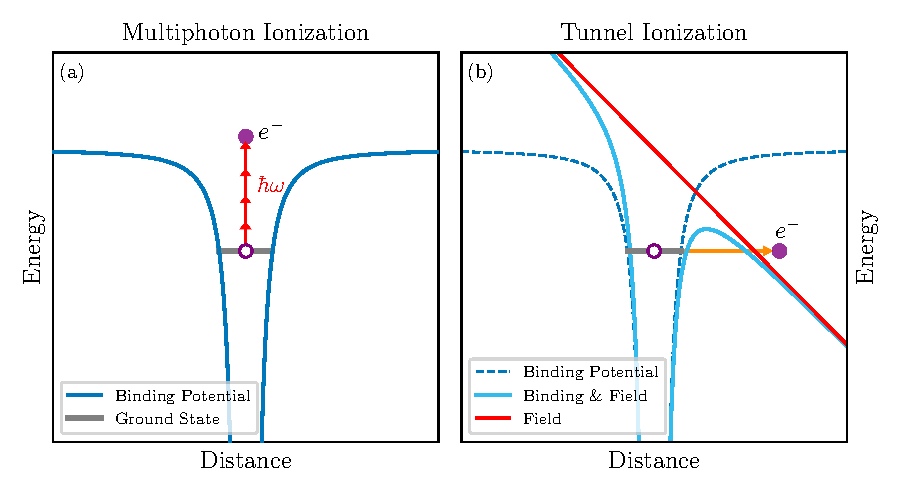
\includegraphics[width=0.9\textwidth]{figures/ATS/MPI_Tunneling.pdf}
	\caption[Schematic of multiphoton and tunnel ionization]{Schematic of multiphoton and tunnel ionization of an atomic in a strong laser field. (a) Multiphoton ionization regime where the electron can absorb multiple photons to reach the continuum and be ionized.  (b) Tunnel ionization regime where the electric field of the dressing laser distorts the atomic binding potential to allow for  bound electron to tunnel through the finite barrier created by the combined atom-field potential.}
	\label{fig:mpi_tunnel}
\end{figure}

In the multiphoton regime, the ionization process can be treated perturbatively, and the physical picture is that the electron is able to absorb multiple photons to gain enough energy to reach the continuum, as shown in figure \ref{fig:mpi_tunnel} (a).  The perturbative treatment means that the ionization probability will be proportional to $I^N$ where $I$ is the intensity of the dressing field and $N$ is the minimum number of photon required to reach the continuum \cite{boydNonlinearOptics2008}.  Absorption of additional photons beyond the minimum number required to ionize is also possible and is know as above threshold ionization (ATI), and was first observed experimentally in 1979 \cite{agostiniFreeFreeTransitionsFollowing1979a}.

In the limit of longer wavelengths, the nonlinear order $N$ increases, and eventually, another process begins to dominate.  Namely, the ionization process in this limit begins to resemble ionization by a static electric field.  This is schematically shown in figure \ref{fig:mpi_tunnel} (b), and this physically corresponds to suppression of the Coulomb binding potential to the point that an electron has a reasonable probability of tunneling through the finite barrier that is created by the combined atomic and electric fields. The low frequency (long wavelength) allows this to happen by giving the electron enough time to tunnel through the barrier each half-cycle of the dressing laser period.  In this regime, the ionization probability no longer follows the perturbative scaling of $I^N$, and it instead follows an exponential scaling in intensity given by $\exp(-2F_0/3\mathcal{E})$ where $F_0$ is related the binding electric field and $\mathcal{E}$ is the dressing electric field \cite{keldyshIonizationFieldStrong1965,changFundamentalsAttosecondOptics2011}. 

To delineate between these two extrema regimes of ionization, a useful parameter is the Keldysh parameter
\begin{equation}
	\label{eqn:keldysh_param}
	\gamma=\sqrt{\frac{I_p}{2 U_p}}\propto\sqrt{\frac{I_p}{I_0 \lambda^2}}
\end{equation}
where $I_p$ is the ionization potential, $U_p$ is the ponderomotive energy, $I_0$ and $\lambda$ are the laser intensity and wavelength \cite{keldyshIonizationFieldStrong1965}.  The Keldysh parameter represents the adiabiticity of the process, and it determines which regime should be considered.  For strong fields at long wavelengths ($\gamma \ll 1$), the electron is able to tunnel ionize each half-cycle of the field because the rate of change of the field is low and the tunneling rate is high.  For weaker fields at shorter wavelengths ($\gamma \gg 1$), the electron has to absorb multiple photons to gain the necessary energy to ionize.

There are generally two methods to calculate the ionization rate in a strong field, PPT \cite{perelomovIonizationAtomsAlternating1986} and ADK \cite{ammosovTunnelIonizationComplex1966}.\footnote{The acronyms stem from the last names of the authors.}  The full details of their derivation will not be reproduced here, but the main results that are pertinent will be discussed.  The PPT model is the more general of the two, and it is generally applicable to calculating the ionization rate and probability for both regimes of strong field ionization. It assumes is derived for a hydrogenic atom and uses effective quantum numbers to generalize to other atoms.  Following the formalism found in \cite{changFundamentalsAttosecondOptics2011}, the rate of ionization $w$ in the PPT model is  
\begin{equation}
	w_{PPT}(\mathcal{E},\omega)=\sum_{q\geq q_{th}}^{\infty}w_q(\mathcal{E},\omega)
\end{equation}
where $w_q$ is the rate for absorbing $q$ photons and $q_{th}=\lceil (I_p + U_p)/\omega \rceil$ is the minimum number of photons required to ionize an electron after including the AC Stark effect.  Assuming the electron is in a state with quantum numbers $n$, $l$, and $m$, The total rate can be written as
\begin{equation}
\label{eqn:PPT_arte}
\begin{aligned}
	w_{PPT}(\mathcal{E},\omega)&=\abs{C_{n^*l^*}}^2 G_{lm} I_p \bigg( \frac{2F_0}{\mathcal{E}} \bigg) ^{2n^*-\lvert m \rvert -1}\bigg(\frac{1}{\sqrt{1+\gamma^2}}\bigg)^{-\lvert m \rvert -1}\\
	&\times \frac{4}{\abs{m} \sqrt{3\pi}}\bigg(\frac{\gamma^2}{1+\gamma^2}\bigg)e^{-\frac{2F_0}{3\mathcal{E}}g(\gamma)}\sum_{q\geq q_{th}}^{\infty}A_q(\omega,\gamma)
\end{aligned}
\end{equation}
where $\mathcal{E}$ is the electric field of the laser,$F_0$ is the binding field strength related to $I_p$, $\gamma$ is the Keldysh parameter, $\abs{C_{n^*l^*}}^2 G_{lm}$ is a constant related to the atom, and the functions $g(\gamma)$ and $A_q(\omega,\gamma)$ are given in \cite{changFundamentalsAttosecondOptics2011}.  Generally speaking, $g(\gamma)$ is a function that approaches unity as $\gamma\rightarrow0$, and $A_q(\omega,\gamma)$  falls off exponentially with $q$ and increases exponentially with $\mathcal{E}$ up to a saturation point related to $I_p$.  In principle this method has a significant advantage in the fact that it is applicable for both regimes of ionization, however evaluation of the infinite sum makes this method computationally expensive. The ionization rate for several atomic species is shown in figure \ref{fig:adk_ppt} (a).

The other main method that is commonly used to calculate the ionization rate is the ADK method \cite{ammosovTunnelIonizationComplex1966}.  This method can be thought of as an extension of the PPT model in the limit of a static field ($\omega\rightarrow0$), where tunneling ionization is the dominant mechanism.  In this limit, all $\gamma$-dependent terms become unity and the resulting rate is given by
\begin{equation}
\label{eqn:ADK_rate}
	w_{ADK} = \abs{C_{n^*l^*}}^2 G_{lm} I_p \bigg( \frac{2F_0}{\mathcal{E}} \bigg) ^{2n^*-\abs{m} -1} e^{-\frac{2F_0}{\mathcal{E}}}.
\end{equation}
This much simpler expression is generally only valid for values $\gamma$ smaller than roughly 0.5, however the ADK model is used in the literature well  beyond this range even though it is known to underestimate the ionization rate \cite{laiExperimentalInvestigationStrongfieldionization2017}.  This mostly likely due to the ease of computation when compared to PPT.  The ADK ionization rate is given for several atomic species in figure \ref{fig:adk_ppt} (a).
\begin{figure}
	\centering
	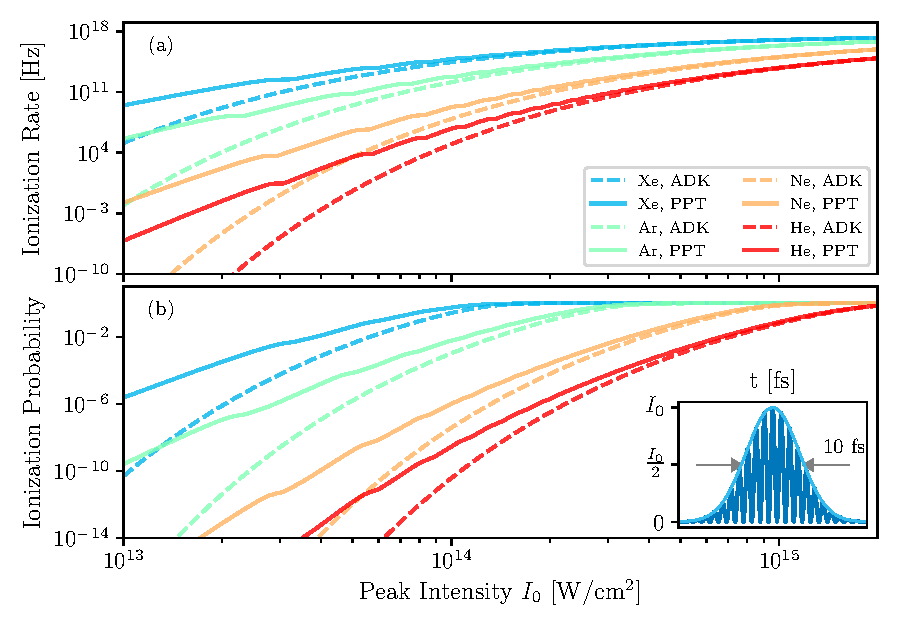
\includegraphics[width=0.8\textwidth]{figures/ATS/ADK_PPT.pdf}
	\caption[ADK and PPT ionization of noble gases]{(a) Ionization rate calculated for various noble gases using both PPT and ADK models as a function of peak intensity for an 800 nm pulse.  (b) Ionization probability integrated through the 800 nm pulse shown in the inset figure as a function of its peak intensity.}
	\label{fig:adk_ppt}
\end{figure}

Generally speaking, both methods have very similar dependence on field strength, and their exponential behaviour means that the ionization rate is limited to a small time window around the peak of the electric field every half-cycle of the laser pulse.  The total ionization probability at a given time $t$ is given by the relation
\begin{equation}
\label{eqn:ion_prob}
	P(t)=1-\exp\bigg(-\int_{-\infty}^{t}w(t')\diff t'\bigg),
\end{equation}
and examples of the ionization probability integrated over an entire pulse is shown in figure \ref{fig:adk_ppt} (b) for several atomic species.

Returning to the DCM parameter $a_1$, it is related to the ionization probability $P(t)$ because the strong field is assumed to deplete the population of the excited discrete state.  The choice of model is dependent upon the dressing laser parameters and the states being considered, but for either model, $a_1$ is given by 
\begin{equation}
\label{eqn:a1_ion_prob}
	a_1(t,\tau) = \exp\bigg(-\int_{0}^{t}w(t' - \tau)\diff t'\bigg).
\end{equation}
This is assuming that the XUV pulse is a $\delta$-function centered at $t=0$.  Effectively, this amplitude attenuates the dipole as a function of time based upon the ionization probability by the dressing pulse, hence this effect is referred to as light-induced attenuation (LIA) of the dipole \cite{chiniSubcycleAcStark2012,chiniCharacterizationApplicationIsolated2012,liaoProbingAutoionizingStates2017}.

Since the dressing pulse is no longer treated as a $\delta$-function, the DCM must be modified to include the form of $a_1$ given in equation \ref{eqn:a1_ion_prob}.  To do this, the initial assumption for the dipole in equation \ref{eqn:piecewise_dipole_t} is extended to include the decrease in amplitude throughout the duration of the dressing pulse, and this is given by
\begin{equation}
\label{eqn:piecewise_dipole_finite_tp}
	d(t, \tau)\propto
	\begin{cases}
		0 & t<0\\
		a_1(t,\tau)i\bigg[\delta(t) + \frac{\Gamma}{2}(q-i)^2 e^{-i\Omega_r t}e^{-\frac{\Gamma}{2}t} \bigg] & t>0.
	\end{cases}
\end{equation}
The cross section can then be calculated by Fourier transforming the dipole and taking the imaginary part.  The dipole in the frequency domain is given by
\begin{equation}
\label{eqn:sigma_a1_finite}
	\tilde{d}(\omega,\tau) = \int_{-\infty}^{\infty}d(t,\tau)e^{i\omega t}\diff t \propto i a_1(0,\tau) + \frac{\Gamma}{2}(q-i)^2 \int_{0}^{\infty}a_1(t,\tau)e^{-i(\omega - \Omega_r) t}e^{-\frac{\Gamma}{2}t}\diff t,
\end{equation}
and the cross section is then
\begin{equation}
\label{eqn:cross_section_a1_finite}
	\sigma(\omega,\tau) \propto \mathrm{Im}[\tilde{d}(\omega,\tau)] \propto a_1(0,\tau)+\mathrm{Im}\bigg[\frac{\Gamma}{2}(q-i)^2 \int_{0}^{\infty}a_1(t,\tau)e^{-i(\omega - \Omega_r) t}e^{-\frac{\Gamma}{2}t}\diff t\bigg].
\end{equation}
The LIA cross section derived here will be used to explain several features in the ATS spectrogram in section \ref{sec:ATS_ar_LIS}. 

\section{Floquet Theory: Light-Induced States}
\label{sec:LIS_Floquet}

A feature that is seen in ATS experiments that is not included in the DCM introduced in the previous section \ref{sec:DCM} are light-induced states (LIS) that arise during temporal overlap between the dressing and XUV pulses.  These were first seen in early ATS experiments in Helium \cite{chenLightinducedStatesAttosecond2012, chiniSubcycleOscillationsVirtual2013}.  In \cite{chenLightinducedStatesAttosecond2012}, the LIS were explained in terms of a Raman-like two-photon process involving the absorption of an XUV photon and either the emission or absorption of a dressing photon to reach a dark state that is dipole-forbidden from the ground state by a single XUV photon. In this case, the LIS would appear in the absorption spectrogram at an energy corresponding to $\pm1$ dressing photon energy from the dark state.

The description of LISs in terms of a Raman-like process starts to break down when the dressing photon energy is close to resonant to a transition between a bright and dark state \cite{wuTheoryStrongfieldAttosecond2016}.  In this regime, it is more appropriate to think of the LIS as arising from the dressed states of the atom in a strong IR dressing field.  To describe this effect, Floquet theory will be introduced in this section to describe a strongly driven two-level system consisting of near resonantly coupled bright and dark states \cite{shirleySolutionSchrOdinger1965,reduzziPolarizationControlAbsorption2015, wuTheoryStrongfieldAttosecond2016}. 

To begin, a two-level system consisting of a bright state $\ket{1}$ and dark state $\ket{2}$ energetically separated by $\omega_0$ is driven by a periodic electric field at fixed delay.  The Hamiltonian of this system is given by 
\begin{equation}
	\hat{H}(t)\rightarrow
	\begin{bmatrix}
	-\frac{\omega_0}{2} & \Omega(t) \\
	\Omega(t) & \frac{\omega_0}{2}
	\end{bmatrix}
\end{equation}
where $\Omega(t)=\mu\mathcal{E}_0\cos(\omega t)=\Omega_0\cos(\omega t)$ in the time-dependent Rabi frequency.  Since this Hamiltonian is periodic, $H(t+2\pi/\omega)=H(t)$, then Floquet theory states that the wave function can be expanded in a periodic basis to take the form
\begin{equation}
	\ket{\psi(t)}=\sum_{f}c_f e^{-i \epsilon_f t}\ket{\phi_f(t)}
\end{equation}
where $c_f$ is a time-independent expansion coefficient and $\ket{\phi_f(t)}$ and $\epsilon_f$ are the Floquet states and energies \cite{shirleySolutionSchrOdinger1965}.  The Floquet states are themselves periodic and satisfy $\ket{\phi_f(t+2\pi/\omega)}=\ket{\phi_f(t)}$.  The importance of representing the wave function in this basis is the fact that the dynamics have been reduced to a trivia phase evolution across each Floquet state that comprises the total wave function.  Thus, solving the time-dependent \Schrodinger equation in this basis simply consists of finding the Floquest states and their energies. This is done by solving the Floquet equations, which are
\begin{equation}
\label{eqn:floquet_eqn}
	\bigg(\hat{H}(t)-i\frac{\partial}{\partial t}\bigg)\ket{\phi_f(t)}=\hat{H}_F\ket{\phi_f(t)}=e^{-t\epsilon_f t}\ket{\phi_f(t)}
\end{equation}
where $\hat{H}_F$ is the Floquet matrix.

To diagonalize the Floquet matrix, a product basis $\ket{\alpha,n}=\ket{\alpha}\otimes\ket{n}$ is used that consists of the product of the bare state basis $\ket{\alpha}=\{\ket{1},\ket{2}\}$ and the Fourier basis $\ket{n}$.  The Fourier basis states are given by
\begin{equation}
	\begin{aligned}
	\ket{n}&=e^{-in\omega t }\\
	\braket{n|f(t)} &= \frac{1}{T}\int_{0}^{T}e^{in\omega t}f(t)\diff t,
	\end{aligned}
\end{equation}
and they represent the Fourier transform of a function $f(t)$ over one period $T=2\pi/\omega$.  Furthermore, since $\omega$ is the driving frequency of the dressing field, the values of $n$ take on integer values and represent photon number.  In this basis, the Floquet equation \ref{eqn:floquet_eqn} can be represented by
\begin{equation}
	\sum_{\beta,m}\braket{\alpha,n|\hat{H}_F|\beta,m}\braket{\beta,m|\phi_{\gamma,l}} = q_{\gamma,l}\braket{\alpha,n|\phi_{\gamma,l}}.
\end{equation}
The matrix elements $\braket{\alpha,n|\hat{H}_F|\beta,m}$ are related to the Fourier transform of the Hamiltonian, $\hat{H}^{[n]}=\braket{n|\hat{H}(t)}$, and they are given by
\begin{equation}
	\braket{\alpha,n|\hat{H}_F|\beta,m} = \hat{H}_{\alpha,\beta}^{[n-m]} + n\omega\delta_{\alpha,\beta}\delta_{n,m}.
\end{equation}

For the two-level system under consideration, the matrix representation of the Floquet Hamiltonian $\hat{H}_F$ in this basis is block tri-diagonal, and it is given by
\begin{equation}
	\hat{H}_F \rightarrow
	\left[
	\begin{smallmatrix}%{cc|cc|cc|cc|cc}
	-2 \omega-\frac{\omega_0}{2} & 0 & 0 & \frac{\Omega_0}{2} & 0 & 0 & 0 & 0 & 0 & 0 \\
	0 & -2 \omega +\frac{\omega_0}{2} & \frac{\Omega_0}{2} & 0 & 0 & 0 & 0 & 0 & 0 & 0 \\%\hline
	0 & \frac{\Omega_0}{2} & -\omega-\frac{\omega_0}{2} & 0 & 0 & \frac{\Omega_0}{2} & 0 & 0 & 0
	& 0 \\
	\frac{\Omega_0}{2} & 0 & 0 & -\omega + \frac{\omega_0}{2} & \frac{\Omega_0}{2} & 0 & 0 & 0 & 0 &
	0 \\ %\hline
	0 & 0 & 0 & \frac{\Omega_0}{2} & -\frac{\omega_0}{2} & 0 & 0 & \frac{\Omega_0}{2} & 0 &
	0 \\
	0 & 0 & \frac{\Omega_0}{2} & 0 & 0 & \frac{\omega_0}{2} & \frac{\Omega_0}{2} & 0 & 0 & 0
	\\ %\hline
	0 & 0 & 0 & 0 & 0 & \frac{\Omega_0}{2} & \omega-\frac{\omega_0}{2} & 0 & 0 &
	\frac{\Omega_0}{2} \\
	0 & 0 & 0 & 0 & \frac{\Omega_0}{2} & 0 & 0 & \omega+\frac{\omega_0}{2} & \frac{\Omega_0}{2} &
	0 \\ %\hline
	0 & 0 & 0 & 0 & 0 & 0 & 0 & \frac{\Omega_0}{2} & 2 \omega-\frac{\omega_0}{2} & 0 \\
	0 & 0 & 0 & 0 & 0 & 0 & \frac{\Omega_0}{2} & 0 & 0 & 2 \omega+\frac{\omega_0}{2} \\
	\end{smallmatrix}
	\right].
\end{equation}
Diagonalizing this matrix enables one to calculate the Floquet energies and states, and this enables the wave function to calculated for any time.  This diagonalization has been done for a system with an energy separation of $\hbar\omega_0=0.875$ eV and photon energy $\hbar\omega=0.867 eV$, and the Floquet energies as a function of Rabi frequency $\Omega_0$ is shown in \ref{fig:floquet_energies}. As can be seen, the Floquet energies are given by two 'ladders' of states separated by $\hbar\omega$ that are centered on each state.

\begin{figure}
	\centering
	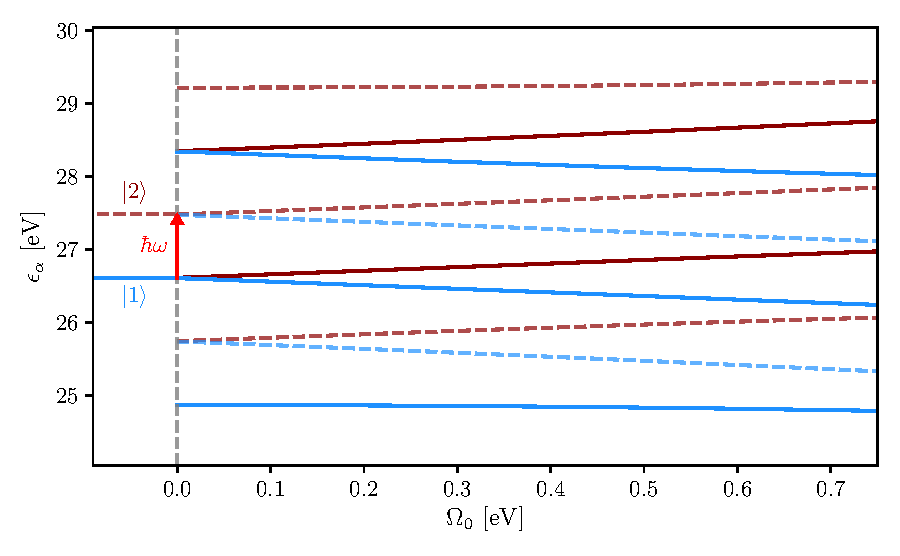
\includegraphics[width=0.8\textwidth]{figures/ATS/floquet_energies.pdf}
	\caption[Floquet energies as a function of Rabi frequency.]{Floquet energies as a function of Rabi frequency.  System consists of a bright state $\ket{1}$ at a energy of 26.605 eV and a dark state $\ket{2}$ at 27.48 eV, and the dressing field of wavelength 1430 nm (shown as a red arrow).  The states which are dipole forbidden from the ground state are shown with dashed lines.  Floquet energies are given by two 'ladders' of states separated by $\hbar\omega$ that are centered on each state.}
	\label{fig:floquet_energies}
\end{figure}

To connect this to ATS experiments, delay-dependence  of the Floquet states must to introduced to calculate the delay-dependent dipole moment.  For the constant field envelope that we have been considering thus far, the delay-dependent Floquet states are given by
\begin{equation}
	\ket{\psi_\alpha(t,\tau)}=e^{-i\epsilon_\alpha t}\sum_{n}e^{-i n\omega(t+\tau)}\ket{\phi_{\alpha,n}}
\end{equation}
where the Floquet states $\ket{\phi_{\alpha,n}}$ and energies $\epsilon_\alpha$ are calculated by diagonalizing $\hat{H}_F$ at a fixed phase $\omega\tau=0$.  Thus, the time- and delay-dependent Floquet states $\ket{\psi_\alpha(t,\tau)}$ can be thought of as a superposition of dressed states that were excited at $t=0$ with a fixed phase of $\omega\tau$.  For an XUV pulse that can be approximated as a $\delta$-function in time, the initial wave function at $t=0$ is given by the superposition
\begin{equation}
	\ket{\Psi(0,\tau)}=\sum_{\alpha}C_{\alpha}(\tau)\ket{\psi_{\alpha}(0,\tau)},
\end{equation}
where $C_\alpha(\tau)=\braket{\psi_\alpha(0,\tau)|\hat{\mu}_X|g} = \sum_n e^{in\omega\tau}\braket{\phi_{\alpha,n}|\hat{\mu}_X|g}$ is the dipole transition matrix element from the ground state $\ket{g}$.  The wave function for $t>0$ is now given by
\begin{equation}
	\ket{\Psi(t,\tau)}=\sum_\alpha C_{\alpha}(\tau)\ket{\psi_{\alpha}(t,\tau)},
\end{equation}
and the time-dependent dipole is
\begin{equation}
\label{eqn:Floquet_dipole}
%\begin{aligned}
%	&=\braket{\Psi(t,\tau)|\hat{\mu}_X|\Psi(t,\tau)}\\
	d(t,\tau) =\sum_{\alpha,m,n}e^{-i(\epsilon_\alpha+m\omega)t}e^{i(n-m)\omega\tau} \braket{\phi_{\alpha,n}|\hat{\mu}_X|g} \braket{g|\hat{\mu}_X|\phi_{\alpha,m}} + c.c.
%\end{aligned}
\end{equation}
From this dipole moment many features that are seen in common ATS spectrograms can be easily understood.  First of all, the exponential term $e^{i(\epsilon_\alpha+n\omega)t}$ means that the dipole will oscillate at frequencies that corresponds to the dressed states of the atom, and therefore, absorption will be observed at photon energies that correspond to the dressed states which are dipole allowed from the ground state. Thus, the LISs that are seen in ATS experiments can be naturally interpreted as probing of the dressed atom.   A second common feature which can be understood from the dipole in equation \ref{eqn:Floquet_dipole} are delay dependent oscillations which arise from the exponential term $e^{i(n-m)\omega\tau}$.  Since only dipole allowed dressed states are probed, this means that only every other state in each  Floquet ladder will contribute to the dipole.  Thus, $n-m$ is even, and the delay-dependent oscillations will be at frequencies of $2\omega$, $4\omega$, etc.  The $2\omega$ oscillations can be interpreted as quantum path interferences between coherently excited dressed states that are separated by $2\omega$ and end up in the same final state \cite{chenQuantumInterferenceAttosecond2013}.  A schematic of the apperance of LIS in the spectrogram is shown in figure \ref{fig:floquet_energies_time_dep} where the Floquet matrix for the two-level system considered previously is diagonalized at each time point and the dressed states are shown.

\begin{figure}
	\centering
	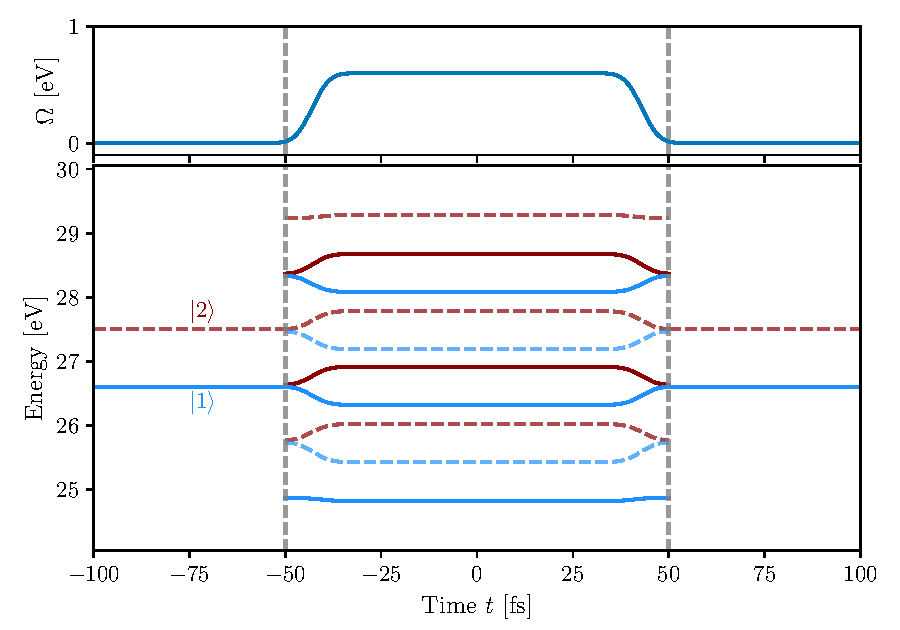
\includegraphics[width=0.8\textwidth]{figures/ATS/floquet_energies_time_dep.pdf}
	\caption[Floquet energies as a function of Rabi frequency and time.]{(a) Rabi frequency as a function of time that represents the strength of the dressing pulse used in this calculation.  (b) Floquet energies as a function of time for the pulse shown in (a). The dressed states which are dipole allowed from the ground state are shown with solid lines, and the dipole forbidden states are shown with dashed lines.  The color corresponds to the two initial states: $\ket{1}$ (bright) and $\ket{2}$ (dark).}
	\label{fig:floquet_energies_time_dep}
\end{figure}


%\section{Time-Dependent \Schrodinger Equation}
%\label{sec:Full_TDSE}

\section{Strong-field Transient Absorption in Argon}
\label{sec:ATS_ar}

Now that the theoretical background has been established for studying the dynamics of autoionizing states in a strong dressing field, we can turn our attention to the experimental study that was conducted using ATS.  The intent of this work was to establish a strong understanding of the dynamics that we should expect to see in chapter \ref{chap:CATS}, where a novel experimental scheme is used to extract a complete picture of the laser-induced dynamics by experimentally measuring the full complex refractive index.

\subsection{Experimental setup}
\label{sec:ATS_ar_exp_setup}

The autoionizing states that will  be studied in this work are the $3s3p^6 np$ states in argon.  The relevant level diagram is shown in figure \ref{fig:fano_level_diagram}, and a table of the resonance parameters is shown in table \ref{table:fano_params}.   This series of states were chosen because they are located energetically in a regime that is easily accessible by HHG sources. The ground state photoabsorption cross section for these states can be calculated using Fano's original theory, equation \ref{eqn:sigma_pcs}, and this is plotted for the resonance parameters of interest in figure \ref{fig:fano_gs_pcs}.  The non-resonant background absorption used in the calculation for figure \ref{fig:fano_gs_pcs} is interpolated from scattering factors available from CXRO \cite{henkeXRayInteractionsPhotoabsorption1993}.  The imaginary part of the scattering factor is related to the photoabsorption cross section by the relationship
\begin{equation}
	\label{eqn:imaginary_scattering_factor}
	\sigma_{\mathrm{NR}}=2 r_0 \lambda f_2,
\end{equation}
where $r_0$ is the classical electron radius and $f_2$ is the imaginary part of the scattering factor.  Since the atomic scattering factor from CXRO does not include fine resonance structure, it can only be used as an approximation of the non-resonant contribution to the total cross section.
\begin{table}[]
	\centering
	\begin{tabular}{|ccccc|}
		\hline\hline
		\multicolumn{1}{|c}{}  & $E_r$ [eV]   & $\Gamma$ [eV]   & $q$         & $\rho^2$     \\ \hline
		$3s3p^64p$              & 26.605 & 80.2(7) & -0.286(4) & 0.840(3) \\
		$3s3p^65p$              & 27.994 & 28.5(8) & -0.177(3) & 0.848(3) \\
		$3s3p^66p$              & 28.509 & 12.2(3) & -0.135(9) & 0.852(9) \\
		$3s3p^67p$              & 28.757 & 6.6(1)  & -0.125(4) & 0.846(9) \\
		$3s3p^68p$              & 28.898 & 4.5(2)  & -0.132(4) & 0.77(2)  \\ \hline\hline
	\end{tabular}
	\caption[Parameters of the $3s3p^6np$ Fano resonances in argon]{Parameters of the $3s3p^6np$ Fano resonances in argon. These values were extracted from experimental cross sections, see \cite{caretteMulticonfigurationalHartreeFockClosecoupling2013, wuElectronimpactStudyValence1995, berrahAngulardistributionParametersAndRmatrix1996}.}
	\label{table:fano_params}
\end{table}


\begin{figure}
	\centering
	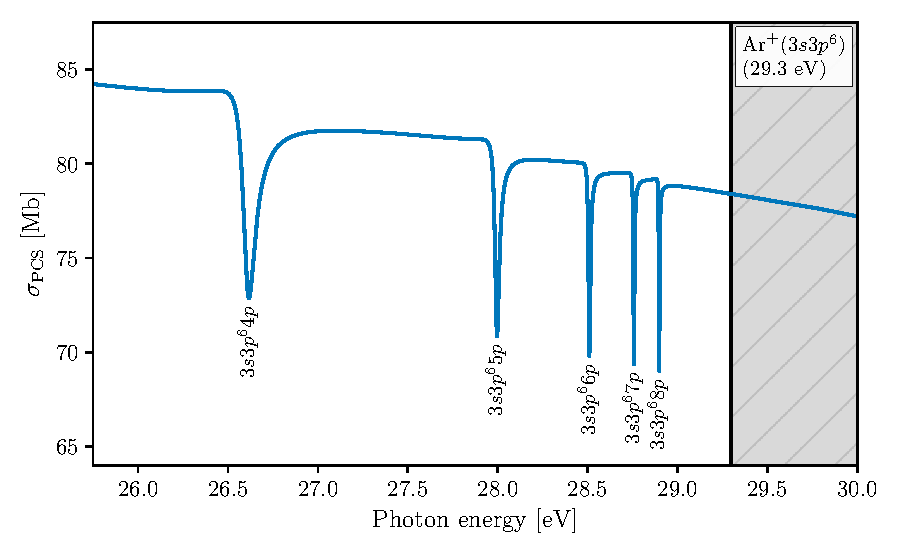
\includegraphics[width=0.8\textwidth]{figures/ATS/fano_GS.pdf}
	\caption[Photoabsorption cross section of the Argon $3s3p^6np$ Fano resonances]{Photoabsorption cross section of the Argon $3s3p^6np$ Fano resonances (blue curve), with only resonances up to $n=8$ shown.  Grey shaded area indicates the energetic region above the $\mathrm{Ar}^+(3s3p^6)$ ionization threshold. Values used to calculate this cross section are shown in Table \ref{table:fano_params}.}
	\label{fig:fano_gs_pcs}
\end{figure}

The TABLe is the experimental apparatus that will be used in all of the experiments described herein, and the relevant optical layout is shown in figure \ref{fig:generation_setup}.  In particular, for these experiments the harmonics are generated using an asymmetric two-color field that allows for the generation of even and odd harmonics. A schematic for how this is implemented, and the resulting XUV harmonic comb, is shown in figure \ref{fig:harmonic_spectrum}.  The harmonic comb that is generated in this way is more energetically dense, and it can be used to more finely sample the ground and excited states of the system.  In particular, there can be light between the harmonics that enable the generation of pseudo-continuum of XUV light.  This feature is important because it enables the observation of several LISs, as will be shown later.

\begin{figure}
	\centering
	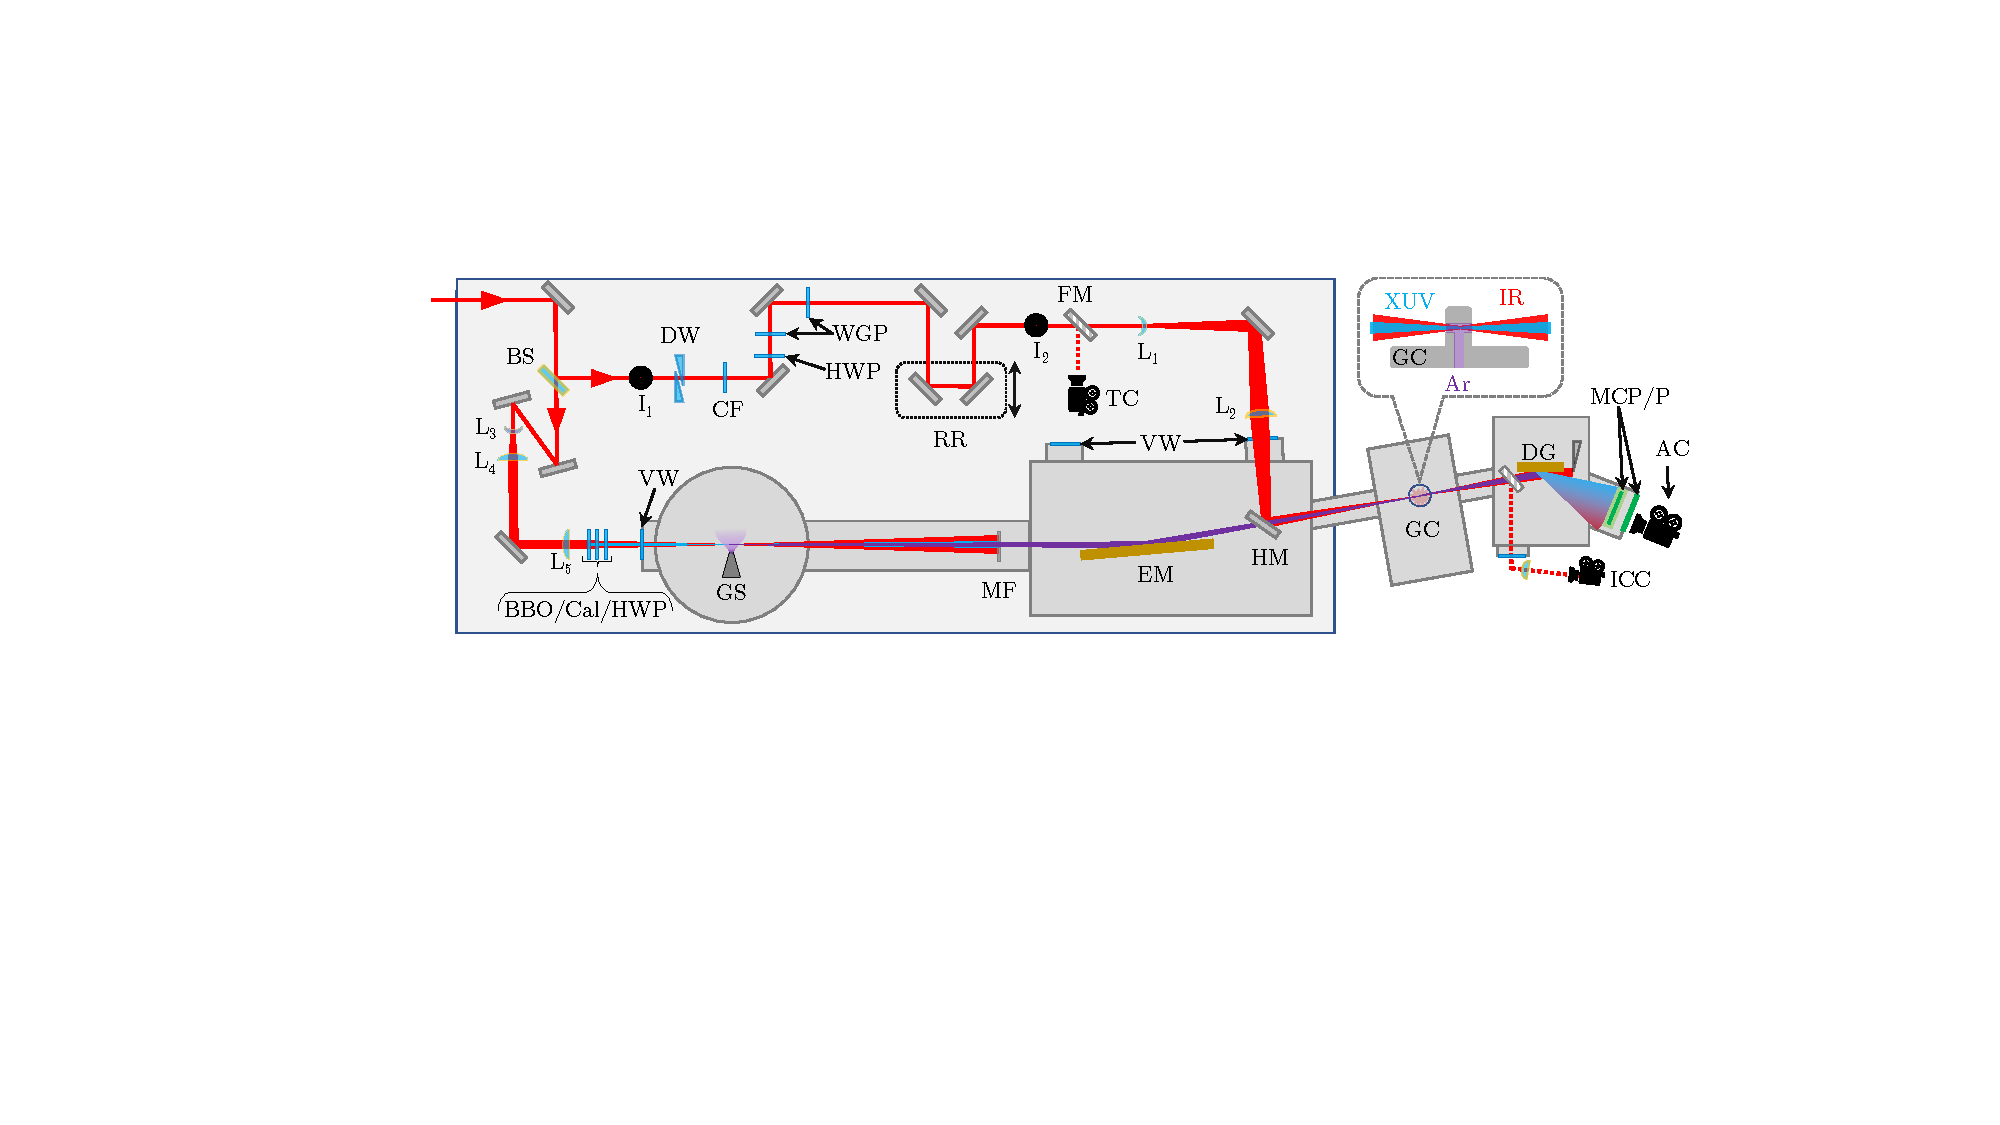
\includegraphics[width=1.0\textwidth]{figures/ATS/ATS_optical_layout.pdf}
	\caption[TABLe experimental setup for ATS experiments]{Schematic of the optical setup for the experiments described in this chapter.  \textbf{BS}: Beamsplitter (Thorlabs BSF20-C), \textbf{I$_{1,2}$}: Irises used for alignment. \textbf{DW}: Delay wedges for fine delay control. \textbf{CF}: Color filter (Thorlabs FELH1000). \textbf{HWP}: Half-wave plate. \textbf{WGP}: Wire grid polarizer. \textbf{RR}: Retro reflector for coarse delay adjustment.  \textbf{FM}: Flip mirror. \textbf{TC}: Thermal camera used for alignment.  \textbf{L$_1$}: $f=-300$ mm lens (Thorlabs LF1015-C). \textbf{L$_2$}: $f=500$ mm lens (Thorlabs LA1380-C). \textbf{VW}: Vacuum window, 3 mm CaF$_2$, \textbf{HM}: Hole mirror with 10 mm hole.  \textbf{L$_3$}: $f=-400$ mm lens.  \textbf{L$_4$}: $f=500$ mm lens. \textbf{L$_5$}: $f=400$ mm lens.  \textbf{BBO}: Second-harmonic generation crystal.  \textbf{Cal}: Calcite. \textbf{GS}: Gas source for HHG. \textbf{MF}: Aluminum filter. \textbf{EM}: Ellipsoidal mirror. \textbf{GC}: Gas cell. \textbf{RM}: Removable mirror for \textit{in-situ} diagnotics.    \textbf{ICC}: camera for \textit{in-situ} diagnotics. \textbf{DG}: VLS diffraction grating. \textbf{BB}: Baffles to block zero order diffraction.  \textbf{MCP/P}: Microchannel plate and phosphor.  \textbf{AC}: Andor Neo 5.5 CMOS camera.}
	\label{fig:generation_setup}
\end{figure}

Using the typical XUV harmonic source shown in figure \ref{fig:harmonic_spectrum}, the ground state photoabsorption spectrum of the $3s3p^6np$ states can be measured.  This is done by measuring the harmonic spectrum with and without argon gas in the gas cell that is shown in figure \ref{fig:generation_setup}.  From these two measurements, the optical density can be calculated as a function of photon energy $\omega$ using Beer-Lambert's Law as
\begin{equation}
\label{eqn:OD}
	\mathrm{OD}(\omega)=-\log(T(\omega))=-\log\bigg(\frac{I_{\mathrm{on}}}{I_{\mathrm{off}}}\bigg) = \frac{\rho l}{\ln 10}\sigma(\omega),
\end{equation}
where $T(\omega)$ is the transmission, $I_{\mathrm{on (off)}}$ is the spectrum with the gas on (off), $\rho$ is the gas density in the interaction region, $l$ is the length of the interaction region, and $\sigma(\omega)$ is the absorption cross section.  For the gas cell used in these experiments, the length $l$ is fixed by the cell design at 2 mm, and the density $\rho$ is set by the backing pressure of the gas cell to achieve the desirable amount of absorption. 

\begin{figure}
	\centering
	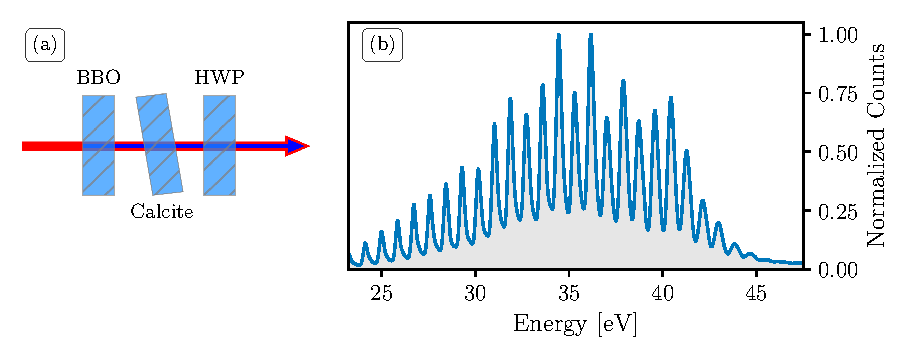
\includegraphics[width=1.0\textwidth]{figures/ATS/harmonic_spectrum_2.pdf}
	\caption[Typical harmonic spectrum used in ATS experiments]{(a) Schematic of $\omega + 2\omega$ scheme to generate even and odd harmonics.  BBO is used to generate $2\omega$. Calcite is used to temporally overlap the two colors at the gas source.  The half wave plate is used to rotate the polarization of the $\omega$ field to match the $2\omega$ field, thereby creating an asymmetric linearly polarized two-color field at the focus. (b) Typical harmonic spectrum used in the experiments described in the chapter.  The harmonics are generated in an $\omega + 2\omega$ scheme where the fundamental wavelength is 1430 nm.  The two-color field used to generate the harmonics has roughly equal intensity in the $\omega$ and $2\omega$ components.}
	\label{fig:harmonic_spectrum}
\end{figure}

The ground state OD of argon measured using the harmonic spectrum in figure \ref{fig:harmonic_spectrum} (b) is shown in figure \ref{fig:fano_fit}.  From this measurement there are three clear features that stand out in the data.  One is an overall decreasing absorption at higher photon energies that is consistent with the non-resonant background absorption that is expected.  This is due to the fact that the absorption cross section decreases monotonically above the ionization potential when neglecting the effect of additional resonances \cite{henkeXRayInteractionsPhotoabsorption1993, sorensenArgon3sAutoionization1994, ogurtsovAutoIonizationStatesArgon1970}.  The second clear feature is an oscillation in the measured OD that is most evident at photon energies above 33 eV.  These oscillations are artifacts of the measurement that arise from one of several sources.  The first possibility is a difference in background counts between the two cases that are being considered (gas on versus gas off).  This can be seen by assuming that the measured spectral amplitudes $\tilde{I}_{\mathrm{on,off}}(\omega)$ differ from the true spectral amplitude  $I_{\mathrm{on,off}}(\omega)$ by a constant amount that can be energy dependent,
\begin{equation}
\label{eqn:measured_approx}
	\begin{aligned}
	\tilde{I}_{\mathrm{on}}(\omega) &= I_{\mathrm{on}}(\omega) + a(\omega) \\
	\tilde{I}_{\mathrm{off}}(\omega) &= I_{\mathrm{off}}(\omega) + b(\omega).
	\end{aligned}
\end{equation}
This means that the measured transmission function $\tilde{T}(\omega)$ will differ from the true transmission function $T(\omega)$ by the relationship
\begin{equation}
	\tilde{T}(\omega) = \frac{\tilde{I}_{\mathrm{on}}}{\tilde{I}_{\mathrm{off}}} = \frac{I_{\mathrm{on}} + a}{I_{\mathrm{off}} + b} \approx T(\omega)\bigg(1 - \frac{a(\omega)}{I_{\mathrm{off}}(\omega)}\bigg) + \frac{b(\omega)}{I_{\mathrm{off}}(\omega)},
\end{equation}
where $a/I_{\mathrm{off}}$ and $b/I_{\mathrm{off}}$ are assumed to be small and only terms up to $\bigO((1/I_{\mathrm{off}})^2)$ are retained.  Since this linear relationship between the measured and true transmission depends upon the harmonic spectral amplitude, one would expect to see modulations in the calculated OD that follow the spacing of the harmonic spectrum.  Thus, for the harmonic spectrum that was used for these measurements that consists of even and odd harmonics, one would expect to see a modulation in the measured OD with a period corresponding to the photon energy of the fundamental wavelength used to generate the harmonic spectrum. This expected modulation at 0.87 eV for a fundamental wavelength of 1430 nm is exactly what is seen in the measured OD in figure \ref{fig:harmonic_spectrum}.  That being said, it is possible to make further assumptions about the stability of the harmonic spectrum in the time between $I_{\mathrm{on}}$ and $I_{\mathrm{off}}$ are measured that can also predict modulations in the measured OD that have a period of the fundamental wavelength.  Regardless of the particular origin of these modulations, they are typically filtered out using some type of band pass frequency filter when analyzing the measured data \cite{ottAttosecondMultidimensionalInterferometry2012, husekElucidatingSurfaceCharge2019}.

The third and final feature that is apparent in the measured OD shown in figure \ref{fig:fano_fit} are the $3s3p^6np$ Fano resonances of interest.  In the measured OD, there is a clear dip in absorption at 26.6 eV with a series of dips that occur at higher energies, and these can be identified as the $4p$, $5p$, and $6p$ resonances.\footnote{Unless stated otherwise, the $3s3p^6np$ will be referred to as the $np$ resonance.} This measured OD can be fit to the photoabsorption cross section calculated using
\begin{equation}
\label{eqn:OD_PSF_fit_func}
	\mathrm{OD}(\omega) = \frac{\rho l}{\ln 10}\bigg[\sigma_{\mathrm{NR}}(\omega) + \sum_{n}\sigma_{n}W_{n}(\omega)\frac{(q_n + \epsilon_n)^2}{\epsilon_{n}^2 + 1}\bigg] \circledast \bigg[\frac{1}{\nu \sqrt{2\pi}}e^{-\frac{(\hbar\omega)^2}{2\nu^2}}\bigg]
\end{equation}
where the sum is over the $np$ states with resonance parameters given by $q_n$ and $\epsilon_{n}=(\hbar\omega-E_{r,n})/(\Gamma_n/2)$, $\circledast$ represents convolution with the Gaussian of standard deviation $\nu$ that is chosen to represent the PSF of the spectrometer, and $\sigma_{n}$, $\nu$, and $\rho l$ are fit parameters.  The function $W_{n}(\omega)$ is a window function that is a convolution of a Gaussian and a boxcar, and this window function is used to limit the range of each resonance \cite{chuTheoryUltrafastAutoionization2010, caretteMulticonfigurationalHartreeFockClosecoupling2013}. In principal, the non-resonant background absorption could be approximated by the cross section from CXRO, however this does not agree well with the experimentally measured OD, as can be seen by the green curve in figure \ref{fig:fano_fit}.  Instead, the non-resonant absorption $\sigma_{\mathrm{NR}}$ is extracted from the measure OD by fitting to an expansion given by
\begin{equation}
\label{eqn:sigma_NR_fit}
	\sigma_{\mathrm{NR}}(\omega) \approx a_0 + a_1(\hbar\omega - E_1) + a_2\mathrm{erfc}(w_2(\hbar\omega - E_2)),
\end{equation}
where $a_i$, $E_i$, and $w_2$ are fit parameters and erfc is the complimentary error function.  This choice of expansion was made for ease of fitting using a least-squares method, and it could easily be replaced by an expansion in a different basis.  


\begin{figure}
	\centering
	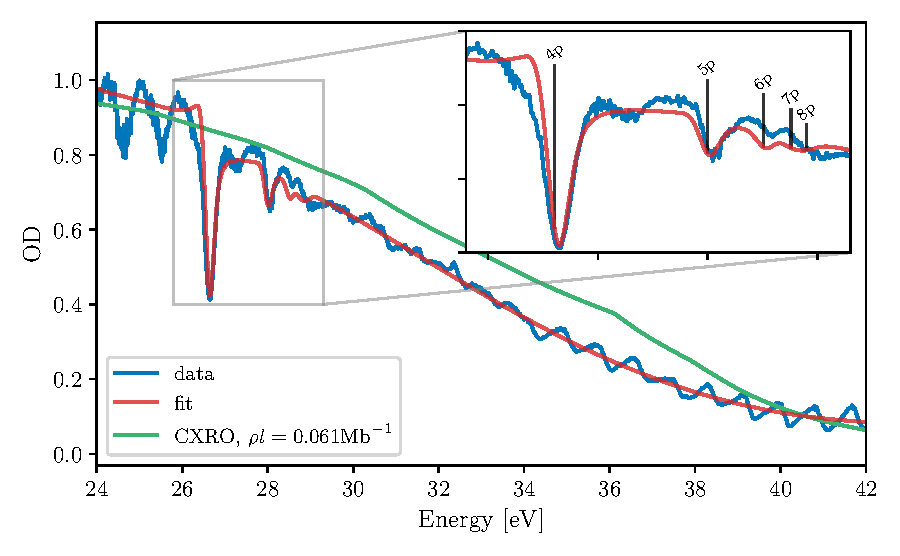
\includegraphics[width=1.0\textwidth]{figures/ATS/fano_fit.pdf}
	\caption{Measured ground state photoabsorption of $3s3p^6np$ Fano resonances.  Blue curve is experimentally measured OD.  Red curve is a fit to the experimental data using equation \ref{eqn:OD_PSF_fit_func}. Inset shows the resonance positions of the $np$ resonances used in the calculation.}
	\label{fig:fano_fit}
\end{figure}

The result of fitting equations \ref{eqn:OD_PSF_fit_func} and \ref{eqn:sigma_NR_fit} to the experimental data is shown as the red line in figure \ref{fig:fano_fit}, and the inset in figure \ref{fig:fano_fit} shows the resonance energy positions of the $4p$ to $8p$ resonances. As can be seen, the $4p$ and $5p$ resonances show reasonably good agreement between the measured OD and the fit, however above the $5p$ resonance it is not possible to clearly identify any resonances. This is likely due to modulations in the measured OD due to either fluctuations in the spectral amplitude of the harmonics or non-zero background counts, as described previously.  That being said, the reasonable agreement between measurement and theory demonstrates the ability to resolve the $np$ resonances, and by applying an appropriate dressing field, the dynamics described previously should be observed.

To that end, the dressing field parameters using the setup detailed in figure \ref{fig:generation_setup} were selected to enable a high dressing intensity given the available laser systems.  This is achieved through the use of a telescope to expand the beam profile to minimize losses on the hole mirror that is used to recombine the XUV and the dressing field. For the experiments described below, the wavelength used is 1430 nm, and the pulse duration is nominally 60 fs.  The range of peak intensities available for this experiment is 0.33 - 42 TW/cm$^{2}$, and this can be finely controlled through the use of a waveplate and wiregrid polarizer.  Further details of the dressing setup are in section \ref{sec:dressing_intensity}.


\subsection{Light-Induced States: Intensity Dependence}
\label{sec:ATS_ar_LIS}

Now that the theoretical background and experimental setup has been thoroughly established, attention can be turned to the experimental results.  To begin, it is useful to first establish the intensity dependence of the features which are observed in the ATS spectrogram, and this will be measured at a fixed delay which corresponds to temporal overlap between the XUV and dressing pulses.  Doing so will develop insight into the nature of resonant effects that are critical for this wavelength dressing field. Following that, the delay-dependent results will be show in section \ref{sec:ATS_ar_delay}. 

The measured intensity dependence of the dressed autoionizing states is shown in figure \ref{fig:dOD_HWP}.  The change in optical density $\Delta\mathrm{OD}$ that is shown in this figure is given by
\begin{equation}
\label{eqn:OD_def}
	\Delta\mathrm{OD} = -\log\bigg(\frac{I_{\mathrm{on}}}{I_{\mathrm{off}}}\bigg) \propto \sigma_{\mathrm{on}} - \sigma_{\mathrm{off}}
\end{equation}
where $I_{\mathrm{on} (\mathrm{off})}$ is the harmonic spectrum with (without) the presence of the dressing field, and it is related to the difference in photoabsorption cross section that the dressing field induces.  As can be seen in figure \ref{fig:dOD_HWP}, there are several distinct features that exhibit strong intensity dependence.  It is expected to observe a change in the photoabsorption in the vicinity of the bright $np$ resonances, however there are additional features that are observed between $np$ states that are dipole allowed from the ground state.  To elucidate this point, a level diagram consisting of both the bright $np$ states and the dark $3s3p^6ns$ and $3s3p^3nd$ states is shown next to the measured $\Delta\mathrm{OD}$ in figure \ref{fig:dOD_HWP}, and the energies of these states are given in table \ref{tab:all_states} \cite{caretteMulticonfigurationalHartreeFockClosecoupling2013, brionThresholdElectronImpact1970, fryarAnalysisEjectedelectronSpectra1976, juretaEnergyAngularAnalysis2016, ogurtsovAutoIonizationStatesArgon1970, sorensenArgon3sAutoionization1994}. Comparing the level diagram to the measured \dod, at the photon energy corresponding to the $4p$, $5p$, and $6p$ resonances there is a similar feature that can be observed.  There is an increase in absorption (red on the color map of figure \ref{fig:dOD_HWP}) that exhibits little shift in photon energy and an amplitude that quickly saturates with increasing peak intensity.  These features will be attributed to suppression of the dipole amplitude from direct ionization of the $np$ states.  The other set of features that can be seen in figure \ref{fig:dOD_HWP} occur at an energies that do not correspond to any of the bright $np$ states, and they generally consist of an increase in absorption (blue on the color map used).  These will be shown to be light-induced states that naturally arise from the dressed atom picture using Floquet theory.  The structure of these light-induced states are critically dependent upon the wavelength of the dressing field, and the wavelength in this case is near-resonant to transitions between bright and dark states.  
\begin{figure}
	\centering
	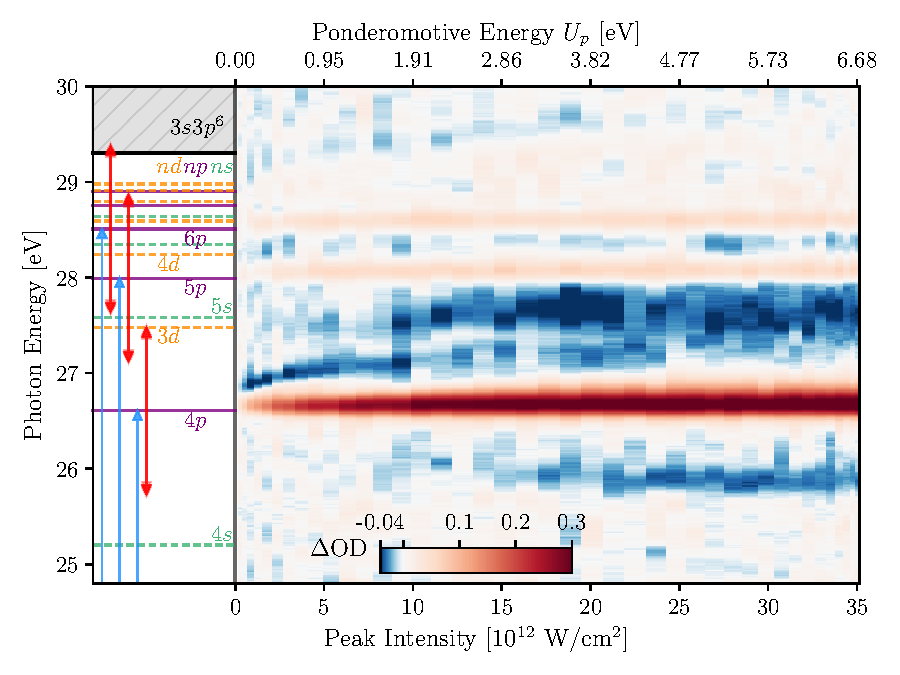
\includegraphics[width=1.0\textwidth]{figures/ATS/dOD_HWP.pdf}
	\caption[Intensity dependence of dressed autoionizing states in Ar]{Intensity dependence of measured $\dod$ near $3s3p^nl$ resonances.  Left portion of shows level diagram with bright (dark) states given by solid (dashed) lines. Red arrows show dressing photon energy, and blue arrows show XUV transitions from ground state.  Right portion of figure shows the measured \dod.}
	\label{fig:dOD_HWP}
\end{figure}

\begin{table}[]
	\centering
	\begin{tabular}{|cc|cc|cc|}
		\hline \hline
		\multicolumn{6}{|c|}{$3s3p^6nl$ excited states}                                               \\ \hline
		Level        & $E_r$ {[}eV{]} & Level        & $E_r$ {[}eV{]} & Level        & $E_r$ {[}eV{]} \\ \hline
		&                &              &                & $3d({}^1\mathrm{D})$ & 27.48          \\
		$4s( {}^1\mathrm{S})$ & 25.2           & $4p({}^1\mathrm{P})$ & 26.605         & $4d({}^1\mathrm{D})$   & 28.24          \\
		$5s( {}^1\mathrm{S})$ & 27.58          & $5p({}^1\mathrm{P})$ & 27.994         & $5d({}^1\mathrm{D})$ & 28.59          \\
		$6s( {}^1\mathrm{S})$ & 28.35          & $6p({}^1\mathrm{P})$ & 28.509         & $6d( {}^1\mathrm{D})$ & 28.80          \\
		$7s( {}^1\mathrm{S})$ & 28.64          & $7p({}^1\mathrm{P})$ & 28.757         & $7d({}^1\mathrm{D})$   & 28.91          \\
		&                & $8p({}^1\mathrm{P})$ & 28.898         & $8d({}^1\mathrm{D})$ & 28.98          \\ \hline \hline
	\end{tabular}
	\caption[Energy of $3s3p^6nl$ states in Ar]{Energy of $3s3p^6nl$ states in Ar \cite{caretteMulticonfigurationalHartreeFockClosecoupling2013, brionThresholdElectronImpact1970, fryarAnalysisEjectedelectronSpectra1976, juretaEnergyAngularAnalysis2016, ogurtsovAutoIonizationStatesArgon1970, sorensenArgon3sAutoionization1994}.}
	\label{tab:all_states}
\end{table}

To further expound upon this, we will first consider the features that arise at the photon energies corresponding to the $np$ resonances.  These increases in absorption can best be understood by utilizing the DCM and LIA theory that was established in sections \ref{sec:DCM} and \ref{sec:LIA}.  Generally speaking, the LIA model describes the suppression of the dipole induced by the XUV pulse through direct ionization of the excited state by the dressing pulse, and the DCM allows for this effect to be analytically calculated for a finite dressing pulse while assuming the XUV pulse is a $\delta$-function in time.  In section \ref{sec:LIA}, it was established that the amplitude $a_1$ is related to the population of the excited state which can be directly ionized by the dressing field, and its relationship to the ionization probability and rate is given be equation \ref{eqn:a1_ion_prob}.  Using equation \ref{eqn:cross_section_a1_finite}, the $\dod$ will be related to the amplitude $a_1$ by
\begin{equation}
\label{eqn:dod_a1}
	\begin{aligned}
		\dod(\omega,\tau) & \propto \sigma_{\mathrm{on}}(\omega,\tau) - \sigma_{\mathrm{off}}(\omega,\tau)\\
		& \propto i\big(a_1(0,\tau)-1\big) + \mathrm{Im}\bigg[\gamma(q-i)^2 \int_{0}^{\infty}\big(a_1(t,\tau) - 1\big)e^{-i\delta t}e^{-\gamma t}\diff t\bigg].
	\end{aligned}
\end{equation}
The effect of $a_1$ on the absorption spectrum can be intuitively understood by looking at limiting cases of this equation.  For the case of $a_1\approx1$ when the field is not intense enough to significantly ionize, $\dod\approx0$ and there is no change in the absorption spectrum as expected.  For the other limiting case of $a_1\approx0$, then $\sigma_{\mathrm{on}}\approx0$ and $\dod\propto - \sigma_{\mathrm{off}}$.  This implies that the effect of $a_1$ is to reduce the contribution that a particular resonance makes to the total cross section, and this provides an intuitive explanation for the features that arise in the at photon energies corresponding to the $np$ resonances in the intensity spectrogram in figure \ref{fig:dOD_HWP}. Specifically, they represent depletion of the $np$ resonances by the dressing pulse until a saturation intensity is reached.

\begin{figure}
	\centering
	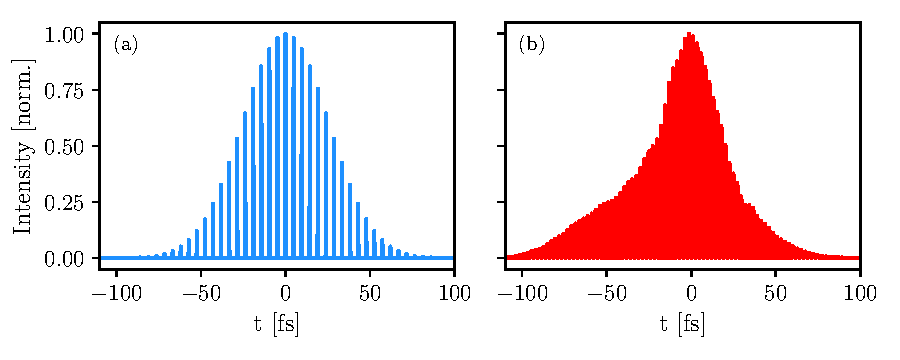
\includegraphics[width=0.9\textwidth]{figures/ATS/fields.pdf}
	\caption[XUV and IR fields used in calculations]{(a) APT used for calculations. Each attosecond burst in the train has a duration 150 as, and the enveloped is Gaussian with a FWHM width of 60 fs.  Since the harmonics consist of both even and odd harmonics, there is a burst only once per cycle.  (b) IR dressing pulse used for calculations, and is the result of a FROG measurement of the output of the TOPAS at the wavelength used for these experiments (1430 nm).}
	\label{fig:fields}
\end{figure}

This qualitative understanding can be made more quantitative by calculating \ref{eqn:dod_a1} for representative XUV and IR dressing pulses.  The pulses that will be used in this calculation are shown in figure \ref{fig:fields}.  Strictly speaking, equation \ref{eqn:dod_a1} only applies for a $\delta$-function XUV pulse, however this restriction can be approximately lifted by averaging the dipole in the time domain with a weighting proportional to the amplitude of the XUV APT $A(t)$,
\begin{equation}
	\label{eqn:dipole_average}
		d_{\mathrm{avg}}(t,\tau)\propto\int_{-\infty}^{\infty}\diff t' A(t')a_1(t-t', \tau)\big[i\delta(t-t') 
		 + i\gamma(q-i)^2 e^{-i\Omega_r (t-t')} e^{-\gamma(t-t')}\Theta(t-t')\big].
\end{equation}
where $\Theta(t)$ is the Heaviside function.  This approximation applies only when each attosecond pulse in the APT can be treated as a $\delta$-function and the dressing pulse has enough intensity to sufficiently reduce the dipole amplitude between each pulse in the APT. The first condition is met because the pulse duration of each pulse in the APT is typically a few hundred as for the laser used to generate the harmonics used in this experiment \cite{orfanosAttosecondPulseMetrology2019, chirlaAttosecondPulseGeneration2011}.  To see that the second condition is met, consider the ionization potential of each of the $np$ states.  For these states, they sit below the $3s3p^6$ threshold by 2.7 eV, 1.31 eV, and 0.8 eV for the $4p$, $5p$, and $6p$ states.


\begin{figure}
	\centering
	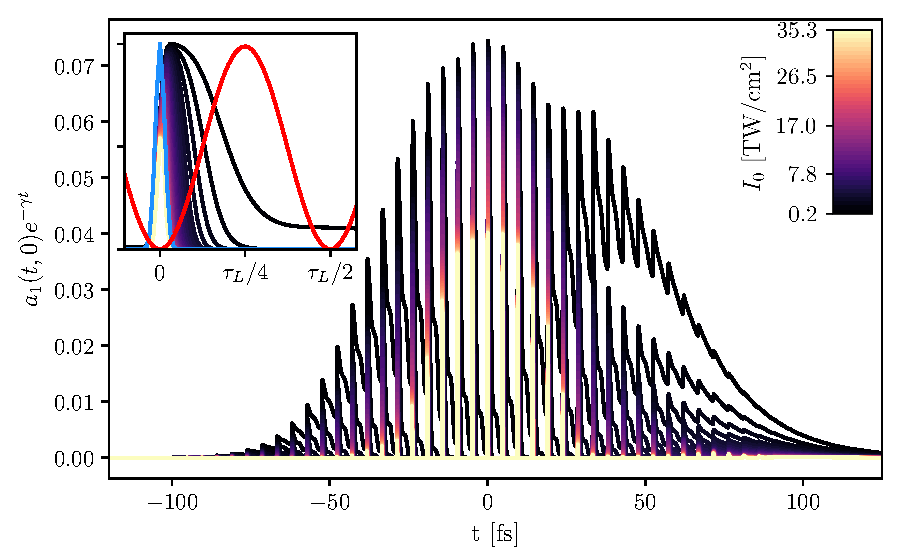
\includegraphics[width=0.9\textwidth]{figures/ATS/a1_t.pdf}
	\caption[Typical harmonic spectrum used in ATS experiments]{dod HWP}
	\label{fig:a1_t_intensity}
\end{figure}

\begin{figure}
	\centering
	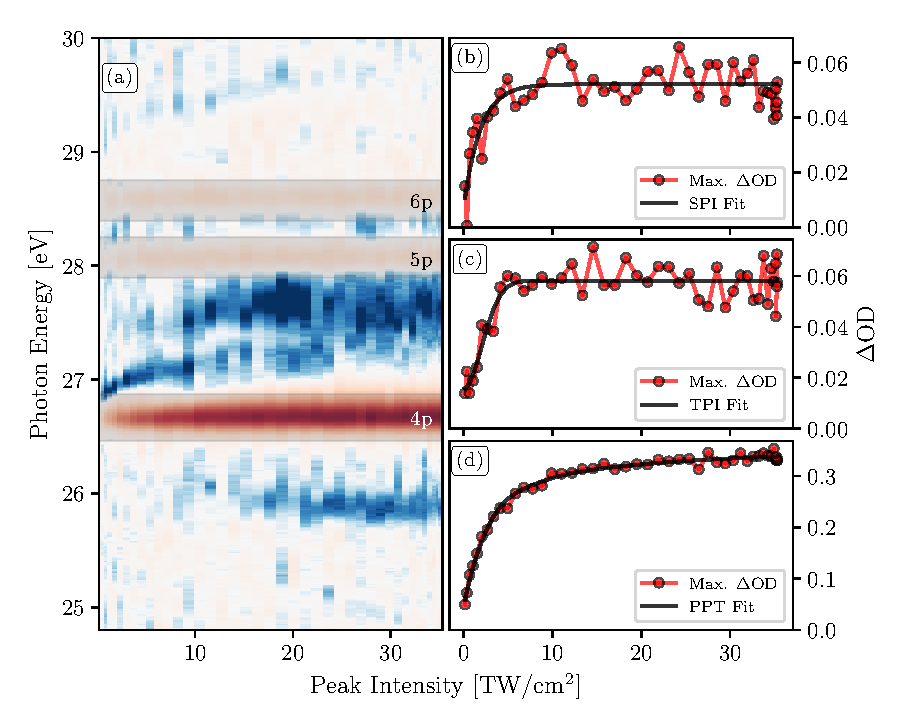
\includegraphics[width=0.9\textwidth]{figures/ATS/np_intensity_dep.pdf}
	\caption[Typical harmonic spectrum used in ATS experiments]{dod HWP}
	\label{fig:np_intensity_dep}
\end{figure}



\begin{table}[]
	\centering
	\begin{tabular}{cccc}
		\toprule
		$\braket{nl|z|n\mathrm{p}}$ &     4p &     5p &     6p \\
		\midrule
		3d & -1.079 &  1.408 & -0.164 \\
		4d &  1.540 & -0.102 &  1.158 \\
		4s &  3.451 &  2.689 &  0.404 \\
		5s &  2.072 &  1.446 &  2.312 \\
		5d &  0.004 &  0.014 &  0.033 \\
		6s &  1.552 &  0.842 &  4.032 \\
		6d &  1.011 &  0.420 &  2.146 \\
		\bottomrule
	\end{tabular}
	\caption{table}
	\label{tab:matrix_elements}
\end{table}


\subsection{Delay Dependence}
\label{sec:ATS_ar_delay}

\section{Conclusion}
\label{sec:ATS_conclusion}

